\documentclass[11pt]{article}
\usepackage{graphicx}
\usepackage{geometry}
\usepackage{setspace}
\usepackage{xcolor}
\usepackage{mathpazo}
%\usepackage{fontspec}
\usepackage[normalem]{ulem} % For underlining text
\usepackage{enumitem} % For resuming lists



% Set font
%\setmainfont{Calibri}

% Set page margins
\geometry{a4paper, margin=1in}



\begin{document}

%\maketitle
\noindent COS20019, Week 4 Lab 

\vspace{0.8cm}

\noindent\textcolor{red}{Please fill in the information below and paste screenshots in the appropriate section. You may}

\vspace{0.1cm}

\noindent\textcolor{red}{add more sections if required.}

\vspace{0.4cm}

\noindent\textbf{Student Name: Abdulswamad Rama Salim} 

\vspace{0.45cm}

\noindent\textbf{Student ID\@: 101229220}

\vspace{1.2cm}

\noindent\underline{\textbf{Build your VPC and Launch a Web Server}}

\vspace{0.6cm}

\noindent\textcolor{red}{Paste screenshot of the \textbf{AWS Management Console} showing your User Account details \\(example shown below). Ensure that your bother screenshots show the menu bar (does not \\need to be expanded).}

\vspace{0.6cm}

\begin{figure}[h]
    \centering
    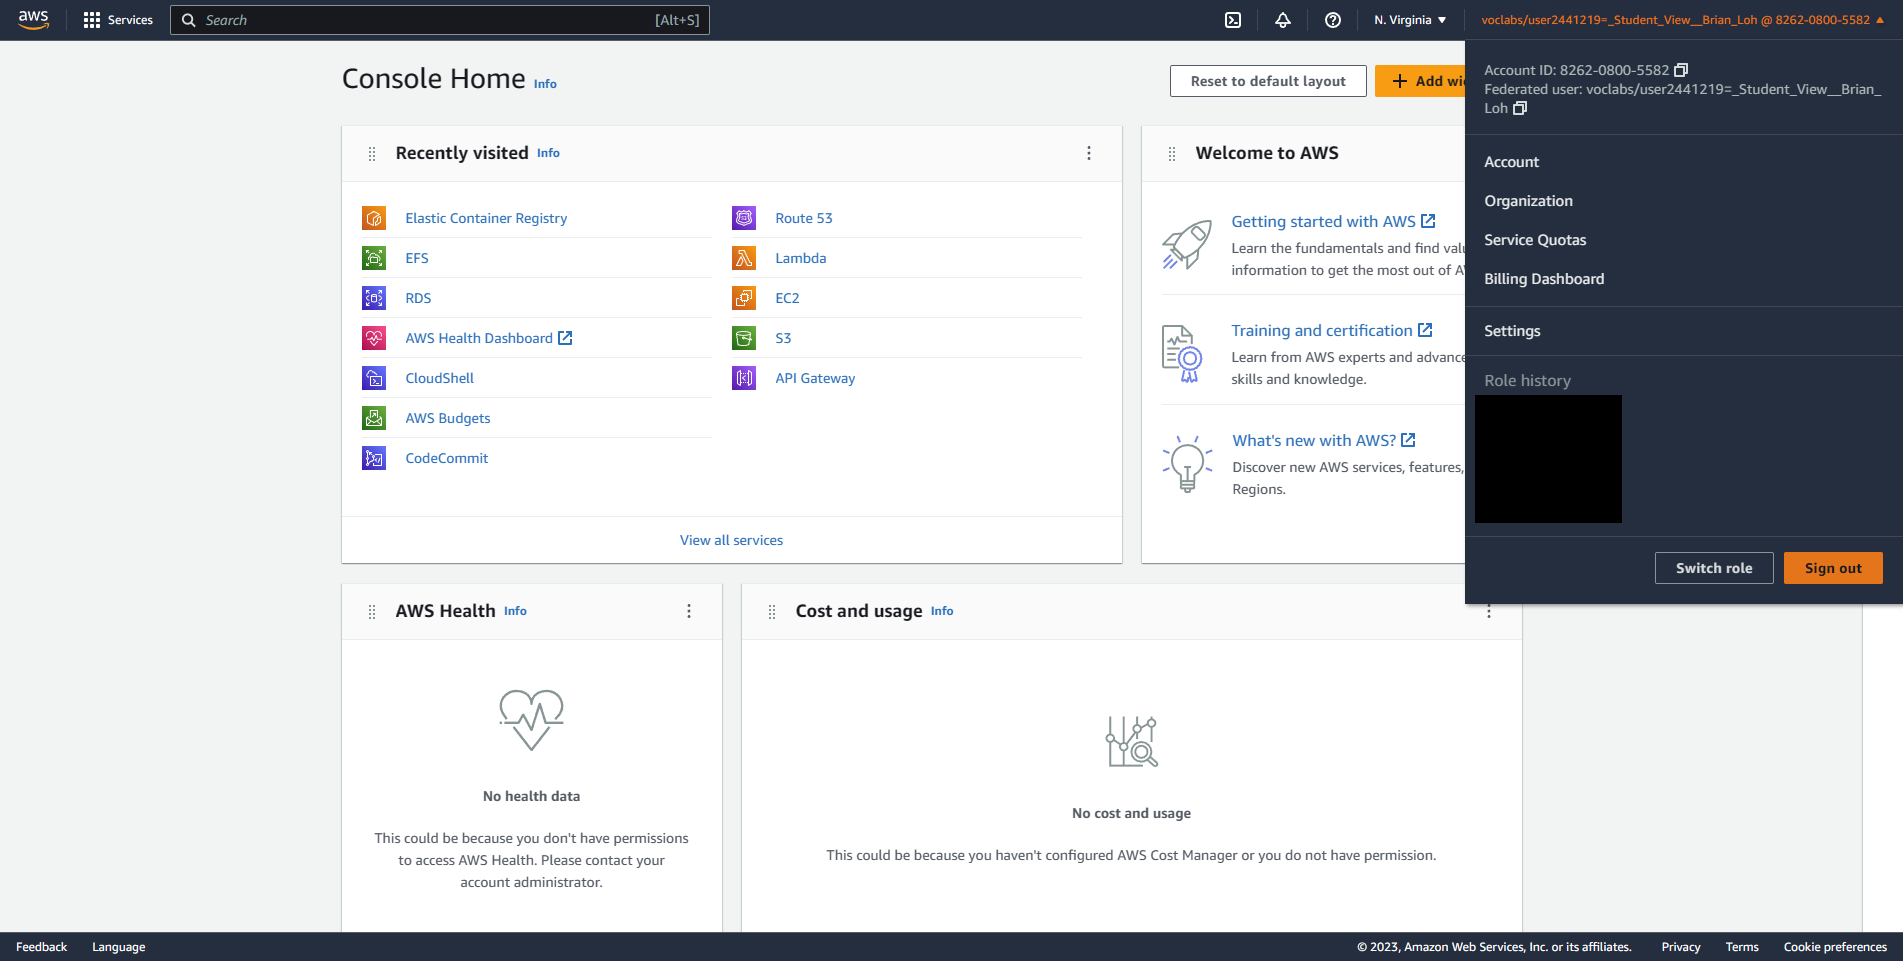
\includegraphics[width=6.2in]{pics/pic.png}
\end{figure}


\vspace{1.5cm}

\newpage

\noindent\underline{Task 1: Create Your VPC}

\begin{enumerate}
    \item Paste screenshot$($s$)$ of the \textbf{Your VPCs} screen (showing existing VPCs) \\
    \vspace{5mm}
    
    
    {\centering
    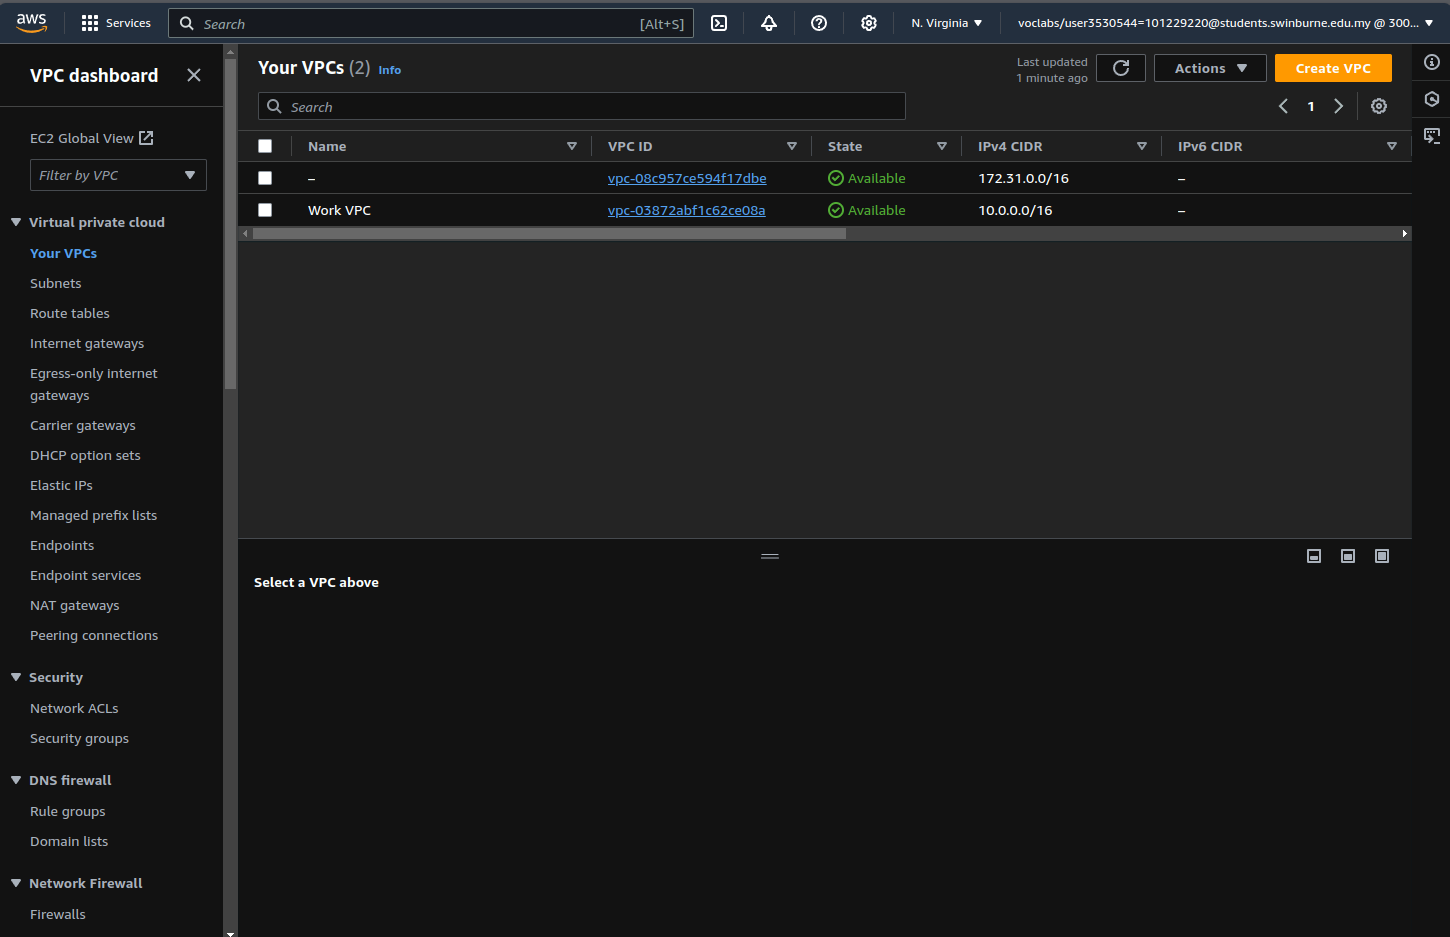
\includegraphics[width=5.8in]{pics/1.png}
    }
    
    \item Paste screenshot$($s$)$ of the \textbf{Create VPC} screen (after entering / choosing the appropriate settings) \\
    \vspace{5mm}

    {\centering
    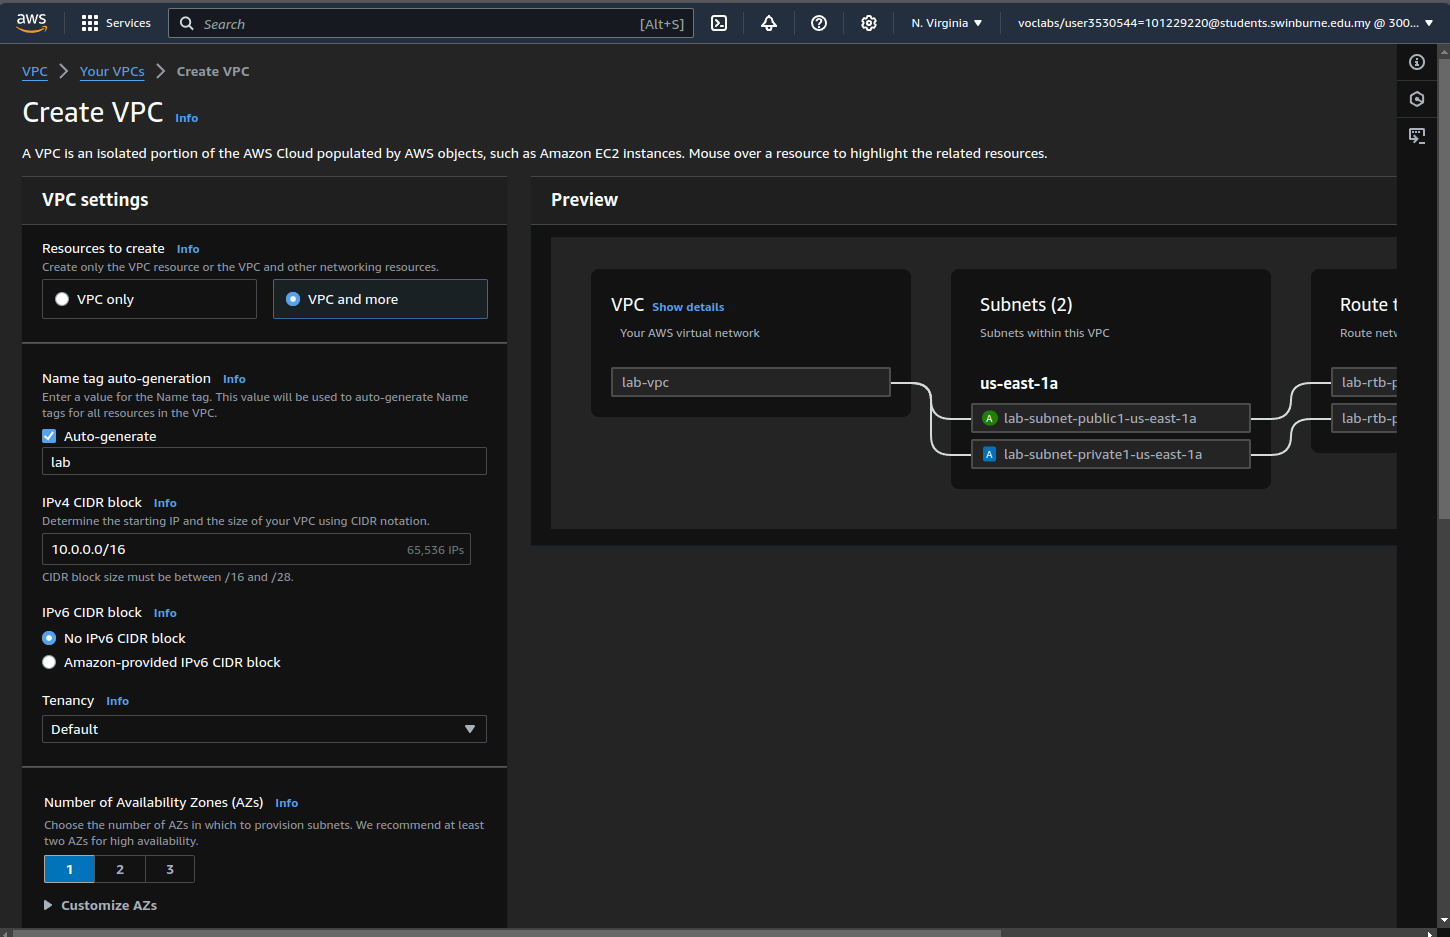
\includegraphics[width=5.8in]{pics/2_a.png}
    }

    {\centering
    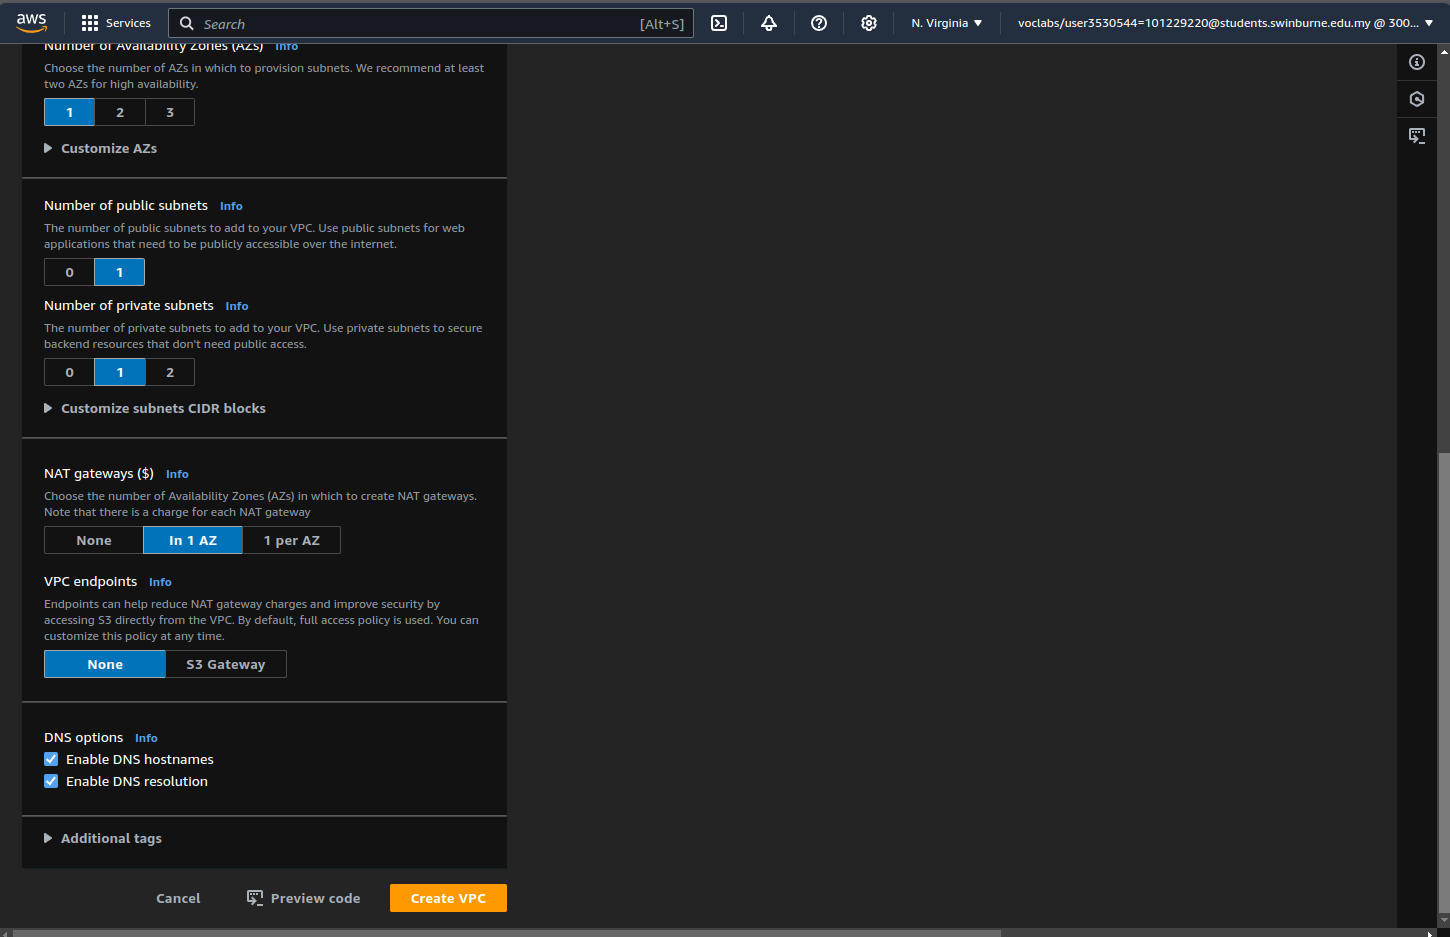
\includegraphics[width=5.8in]{pics/2_b.png}
    }
    
    \vspace{5mm}

    \item Paste screenshot$($s$)$ of the \textbf{View VPC} screen (showing new VPC) \\
    \vspace{5mm}


    {\centering
    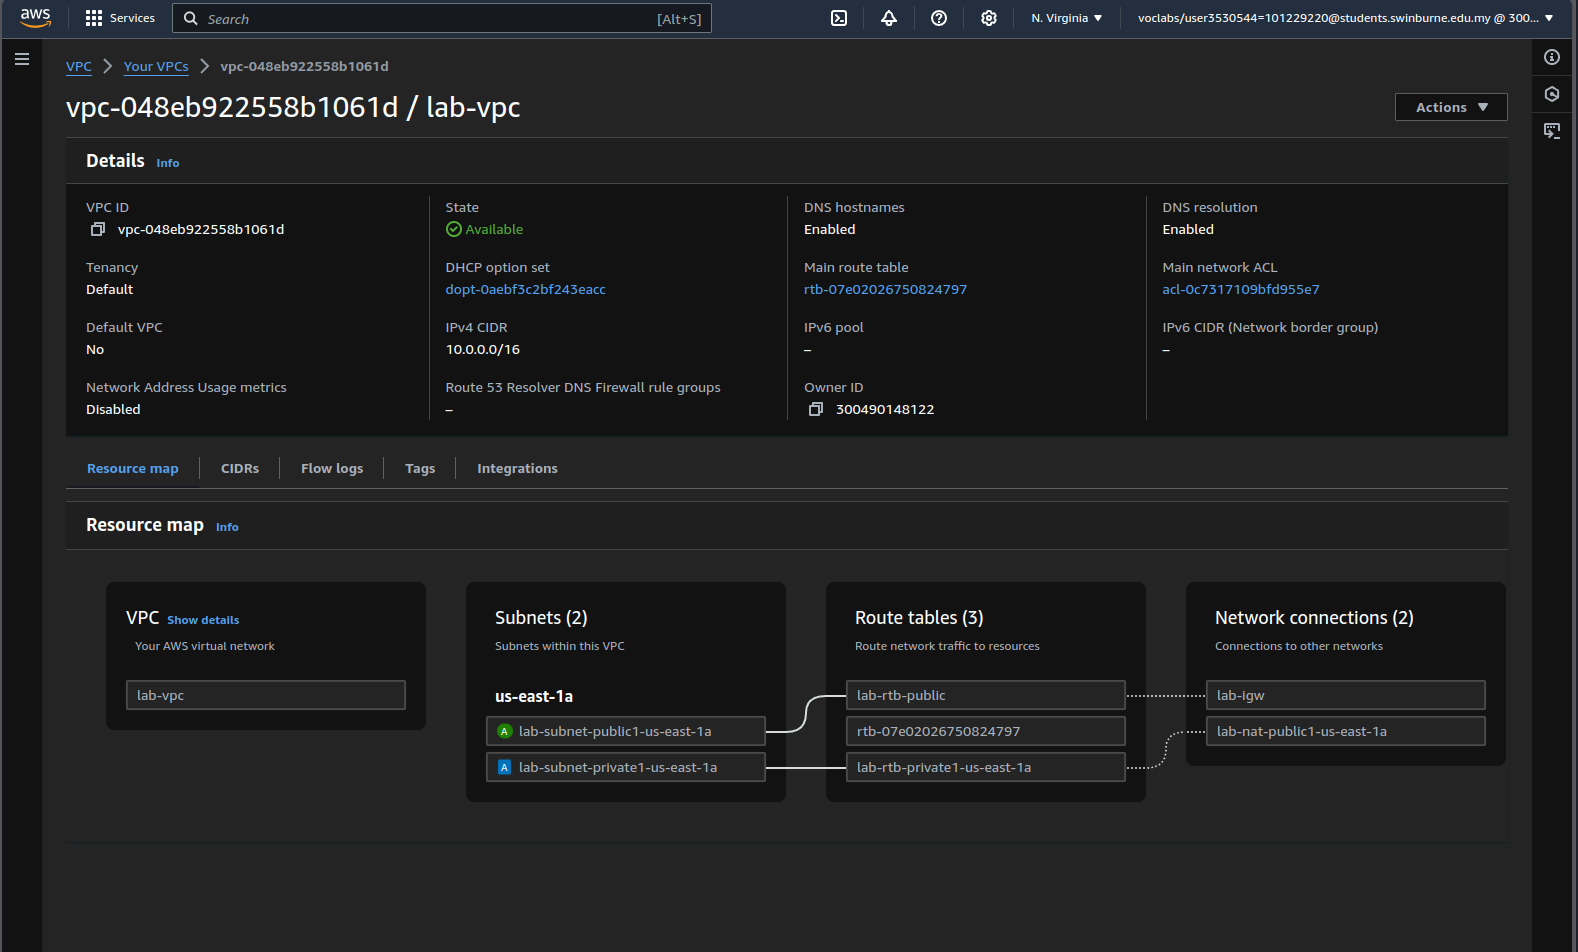
\includegraphics[width=5.8in]{pics/3.png}
    }


\end{enumerate}


\vspace{1cm}

\newpage

\noindent\underline{Task 2: Create Additional Subnets}

\begin{enumerate}[resume]
    \item Paste screenshot$($s$)$ of the \textbf{Subnets} screen (showing existing subnets) \\
    \vspace{5mm}

    {\centering
    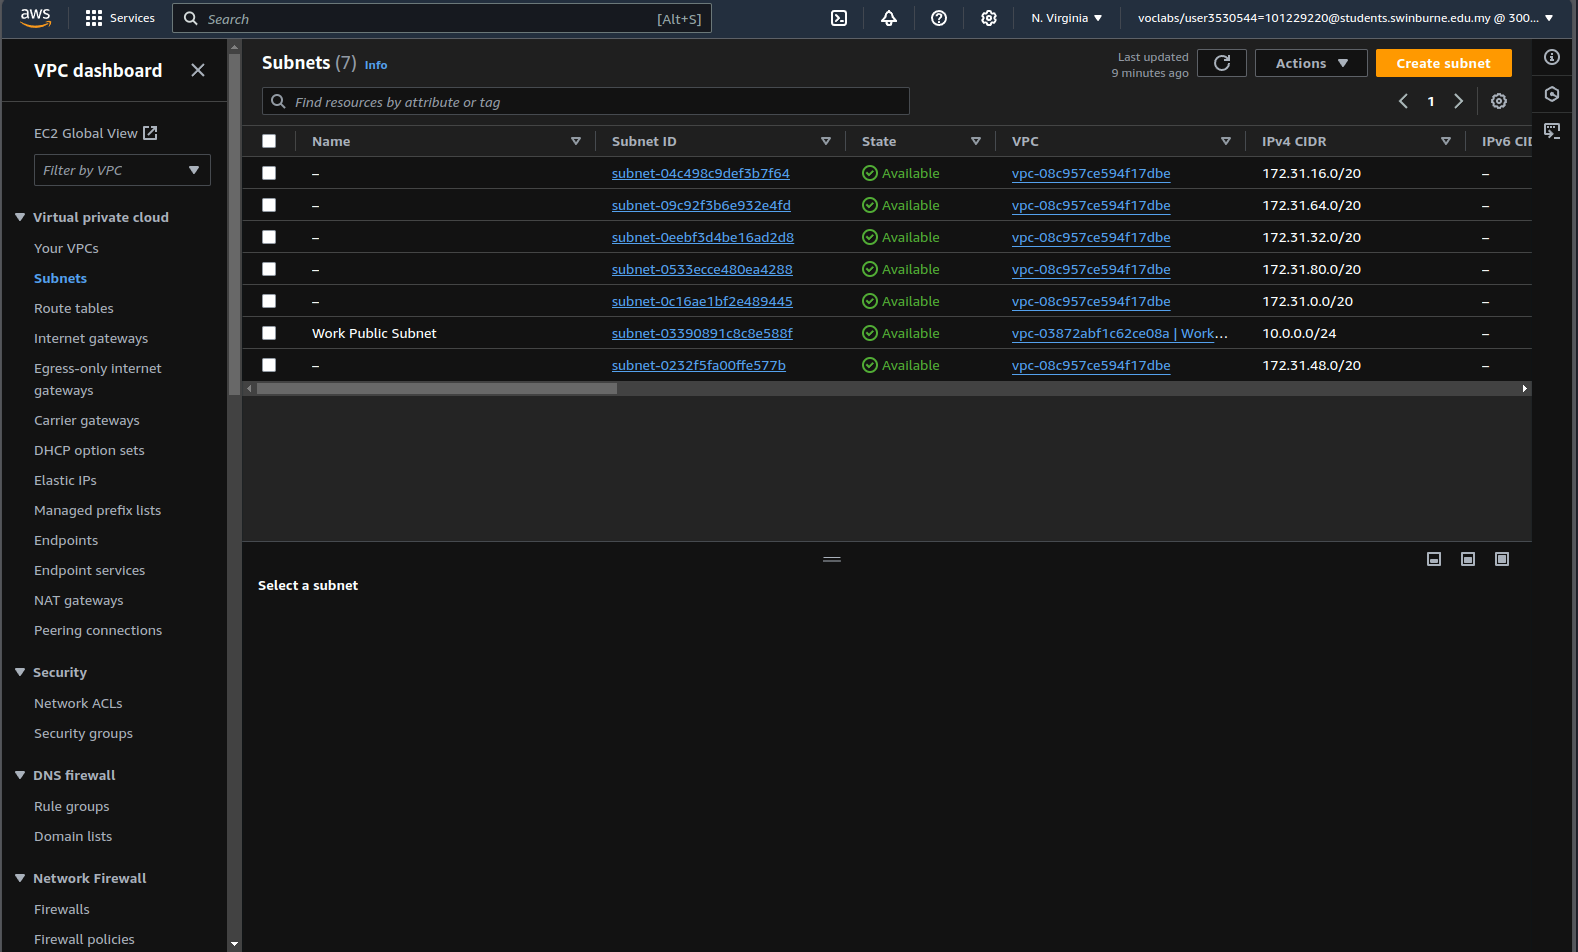
\includegraphics[width=5.8in]{pics/4.png}
    }

    
    \item Paste screenshot$($s$)$ of the \textbf{Create Subnet} screen (after entering / choosing the \\ appropriate settings) \\
    \vspace{2mm}

    {\centering
    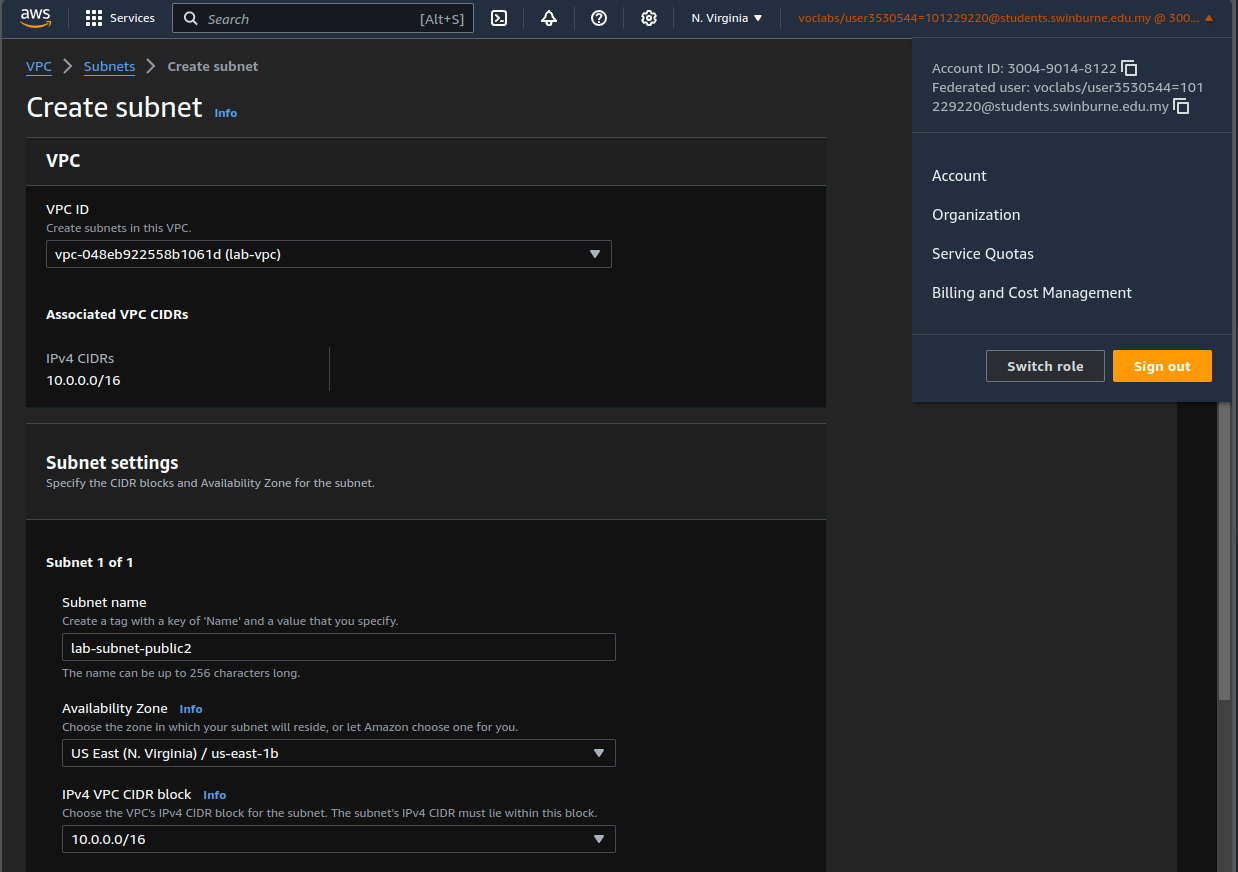
\includegraphics[width=5.8in]{pics/5_a.png}
    }

    {\centering
    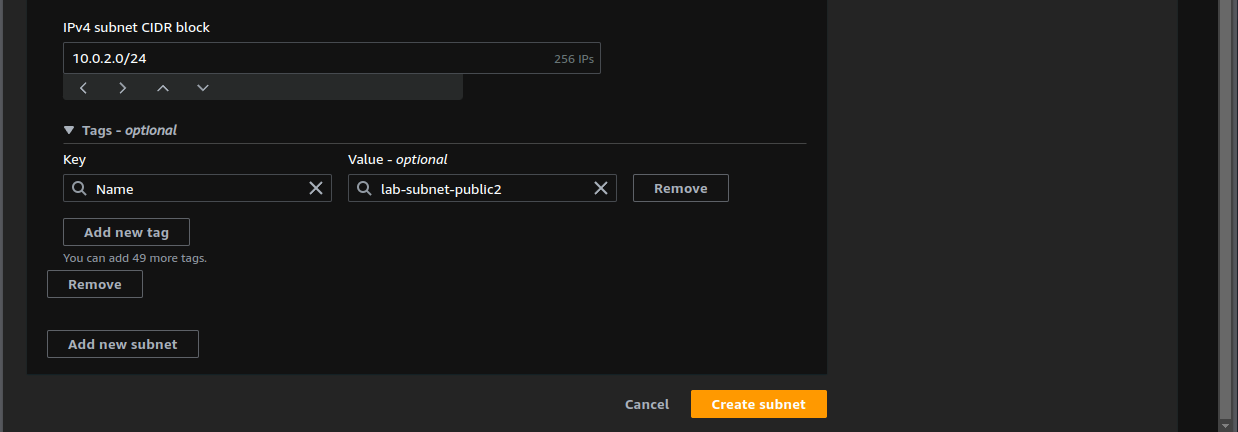
\includegraphics[width=5.8in]{pics/5_b.png}
    }

    
    \item Paste screenshot$($s$)$ of the \textbf{Subnets} screen (showing new public subnet) \\
    \vspace{2mm}

    {\centering
    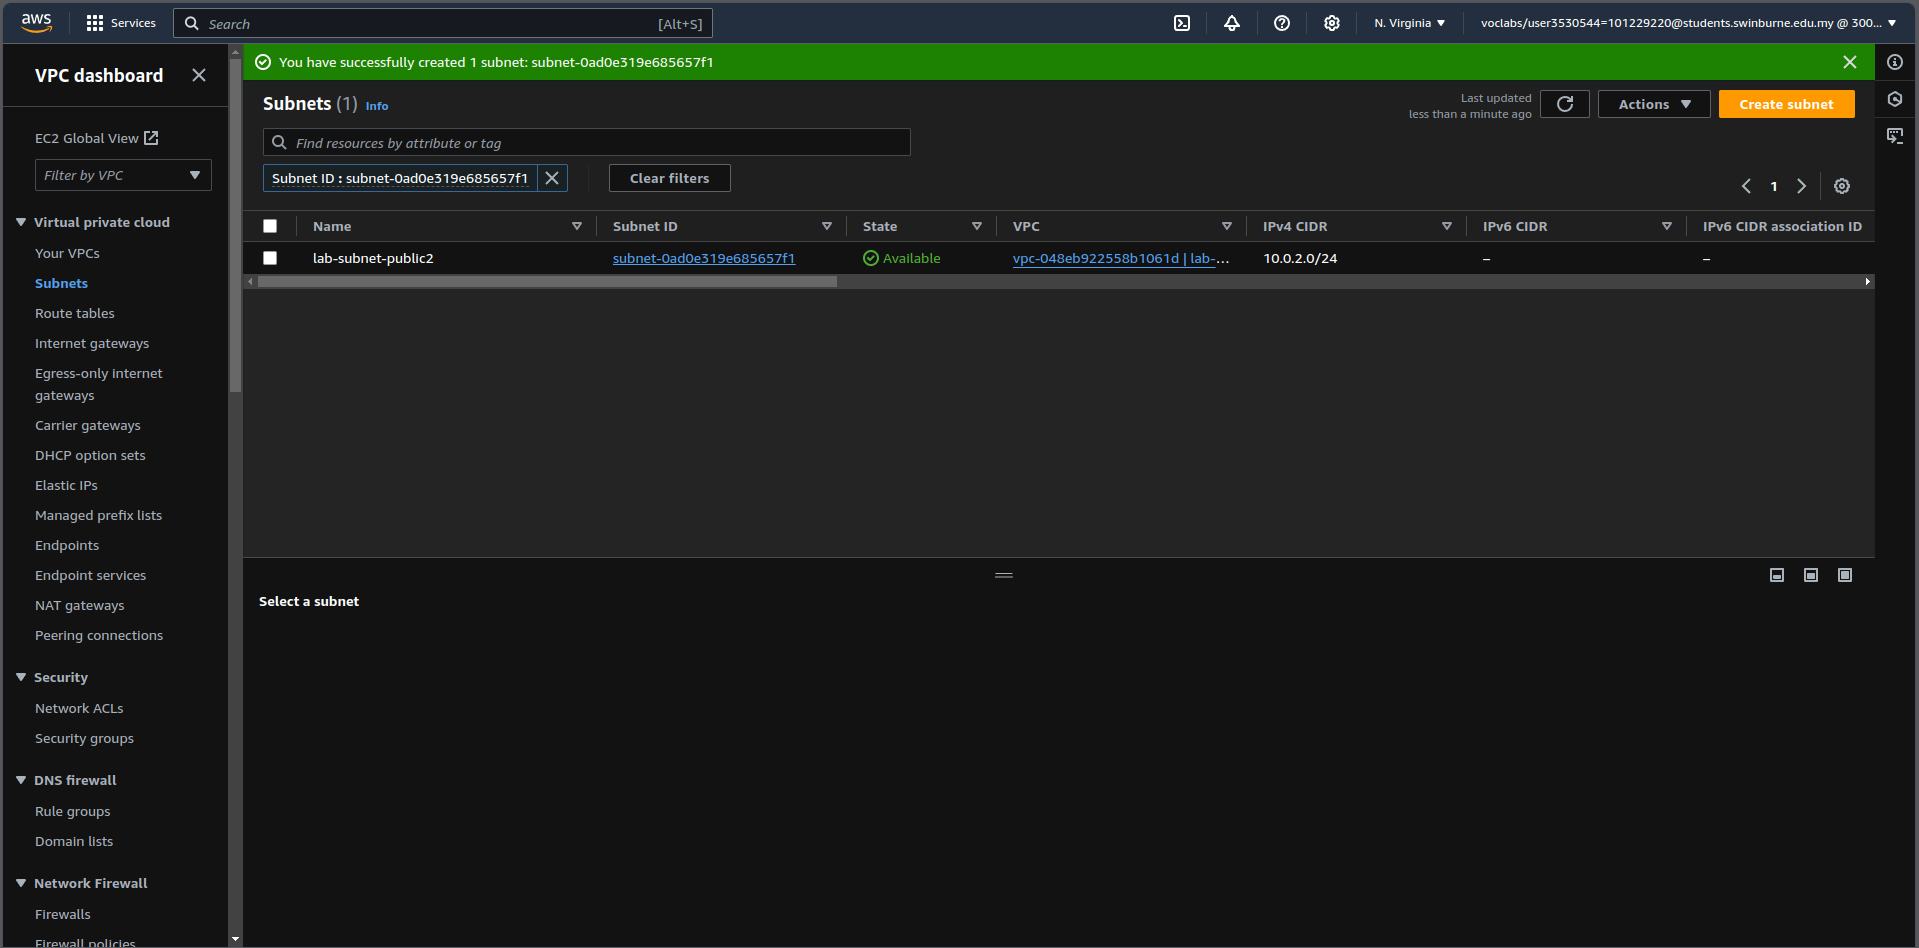
\includegraphics[width=5.8in, height=5.0in]{pics/6.png}
    }
    
    \vspace{50mm}
    \item Paste screenshot$($s$)$ of the \textbf{Create Subnet} screen (after entering / choosing the \\ appropriate settings) \\
    \vspace{-0.02mm}

    {\centering
    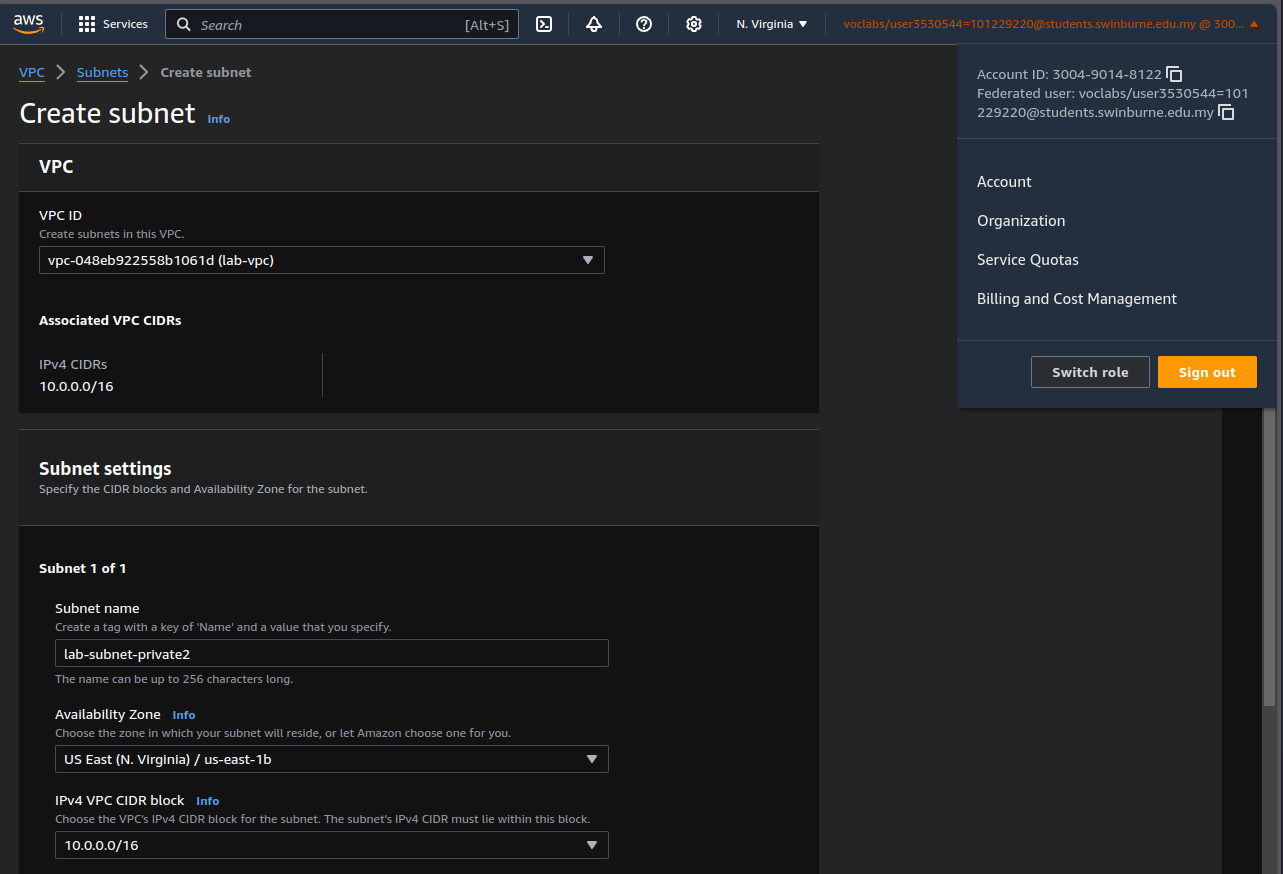
\includegraphics[width=5.8in, height=3.7in]{pics/7a.png}
    }

    \vspace{0.01mm}

    {\centering
    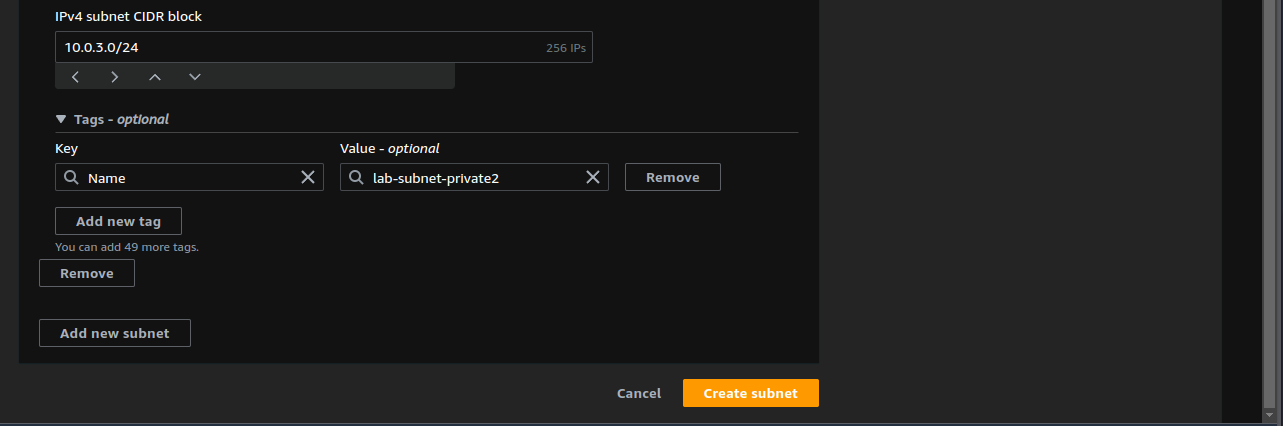
\includegraphics[width=5.8in]{pics/7b.png}
    }

    
    \item Paste screenshot$($s$)$ of the \textbf{Subnets} screen (showing new private subnet) \\
    \vspace{0.01mm}

    {\centering
    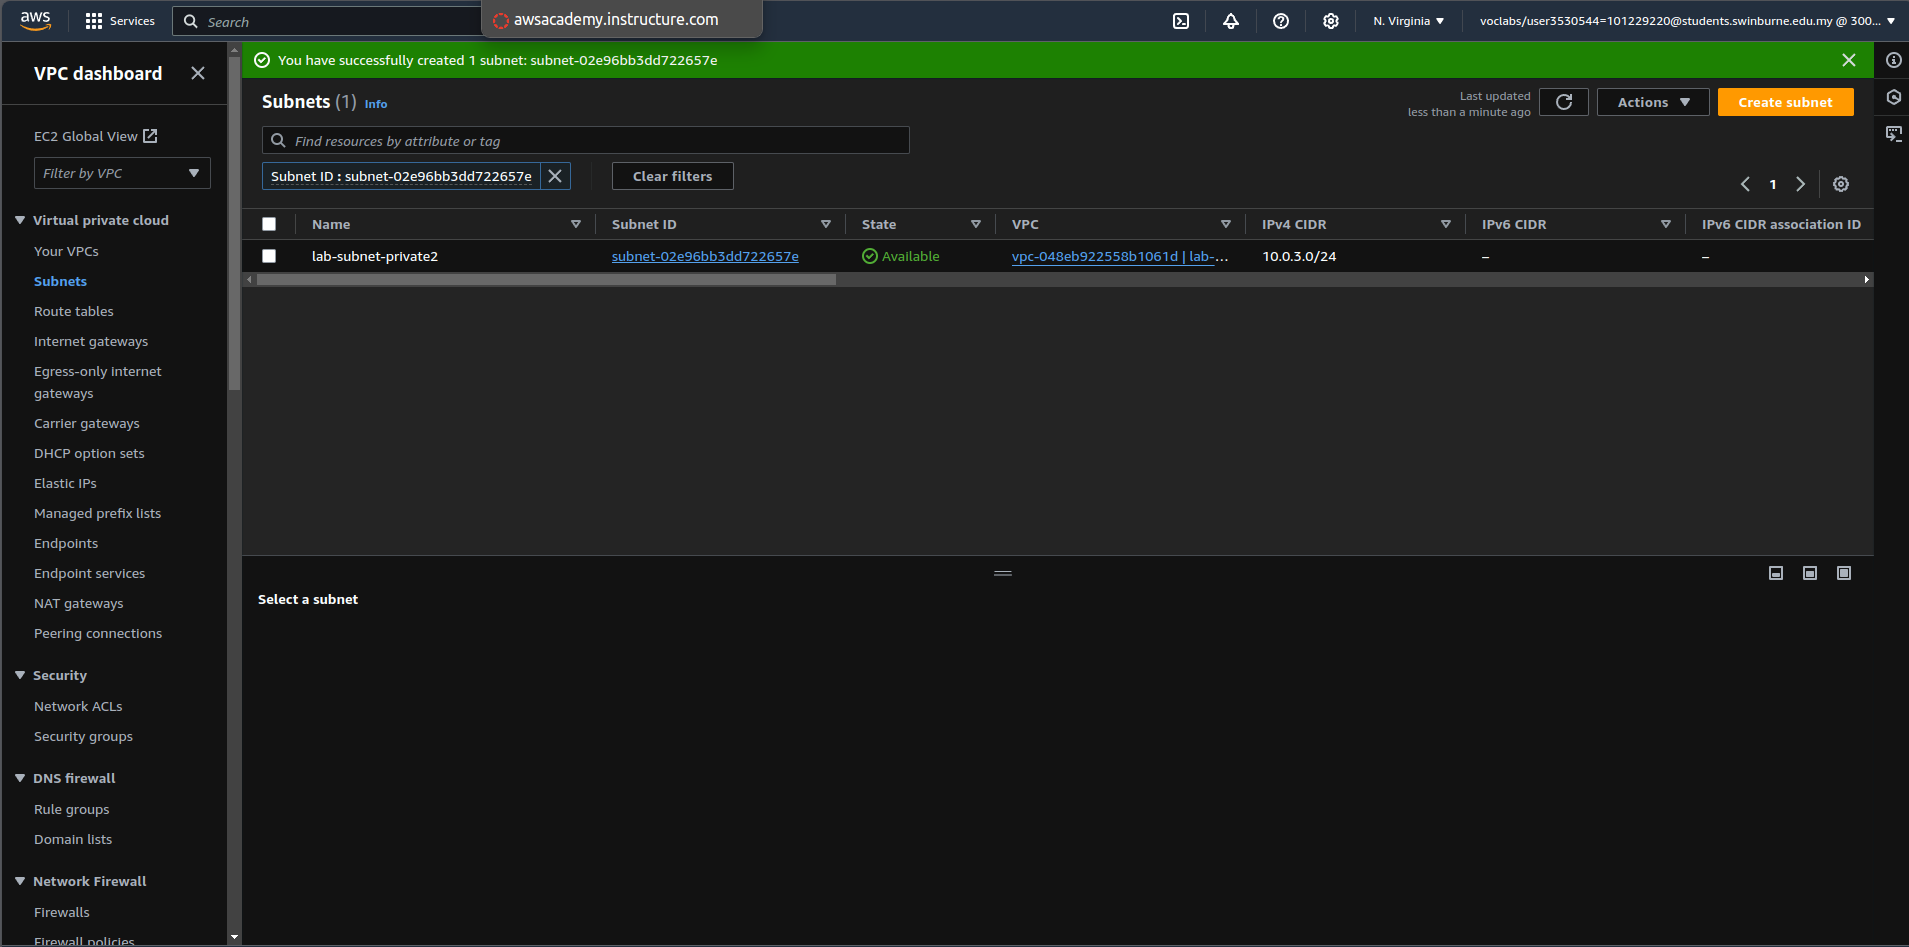
\includegraphics[width=5.8in]{pics/8.png}
    }

    
    \item Paste screenshot$($s$)$  of the \textbf{Subnet associations} tab screen for private route table (after entering / choosing the appropriate settings) \\
    \vspace{5mm}

    {\centering
    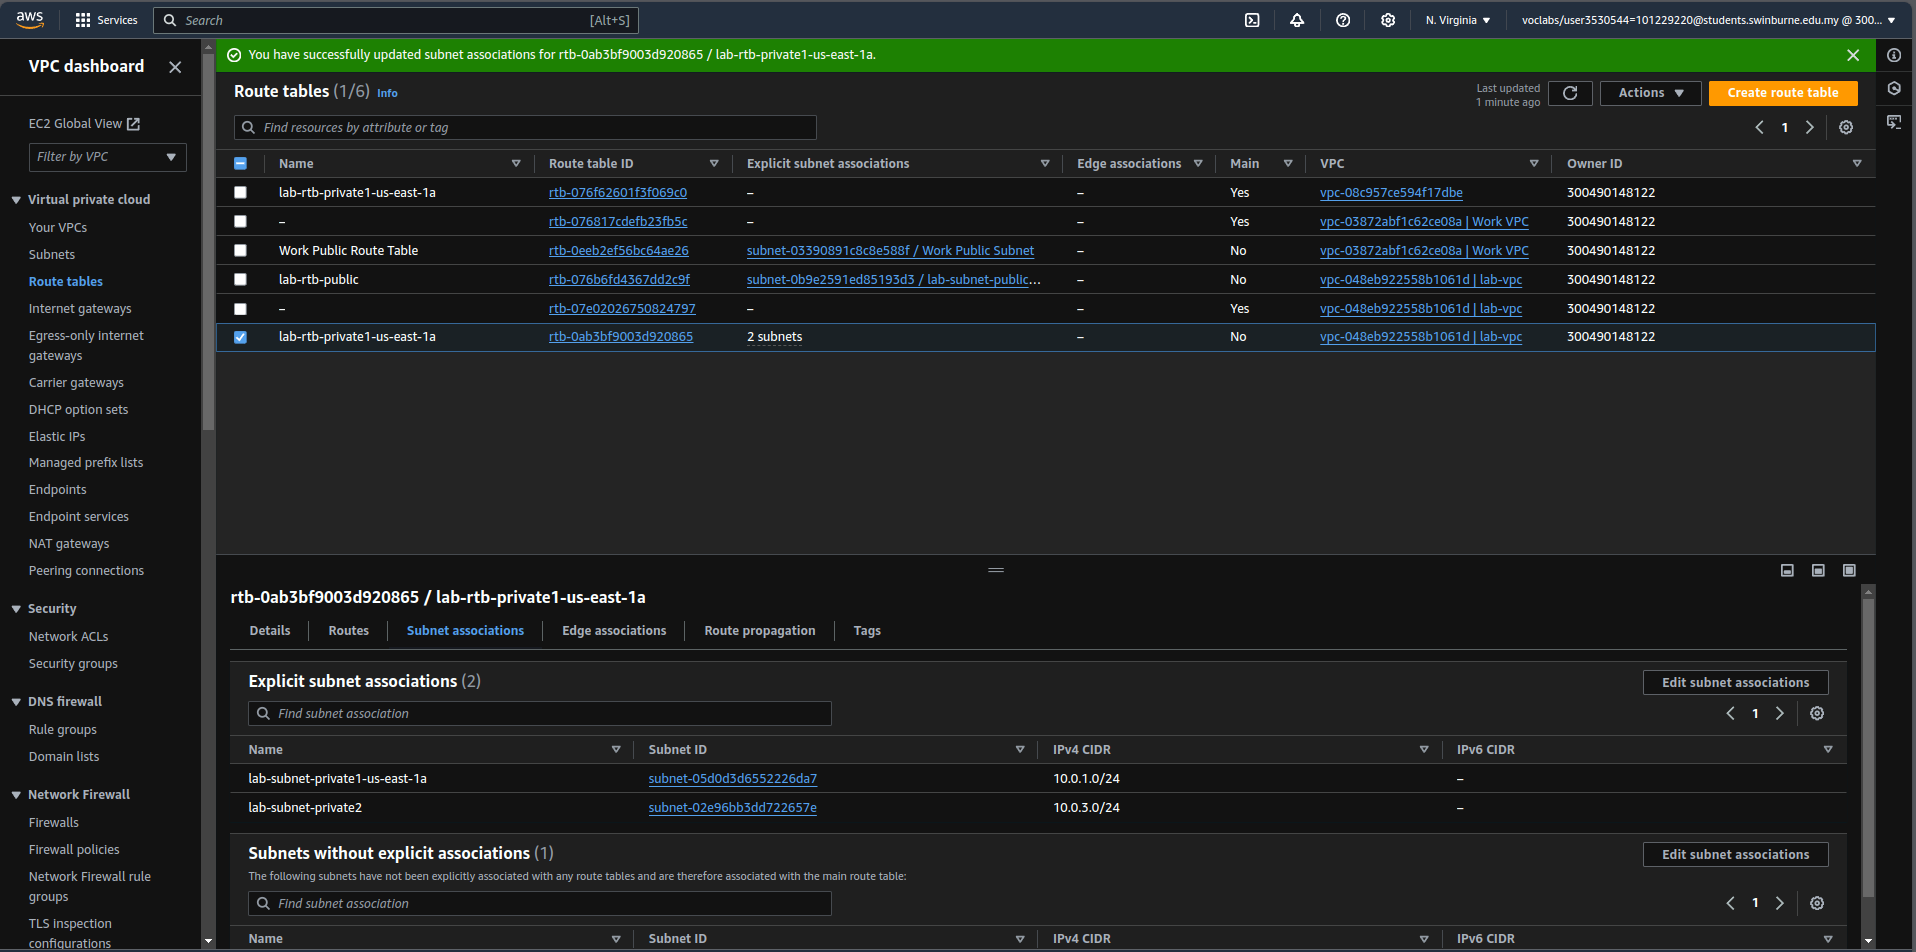
\includegraphics[width=5.8in]{pics/9.png}
    }

    
    \item Paste screenshot$($s$)$ of the \textbf{Subnet associations} tab screen for public route table (after entering / choosing the appropriate settings) \\
    \vspace{5mm}

    {\centering
    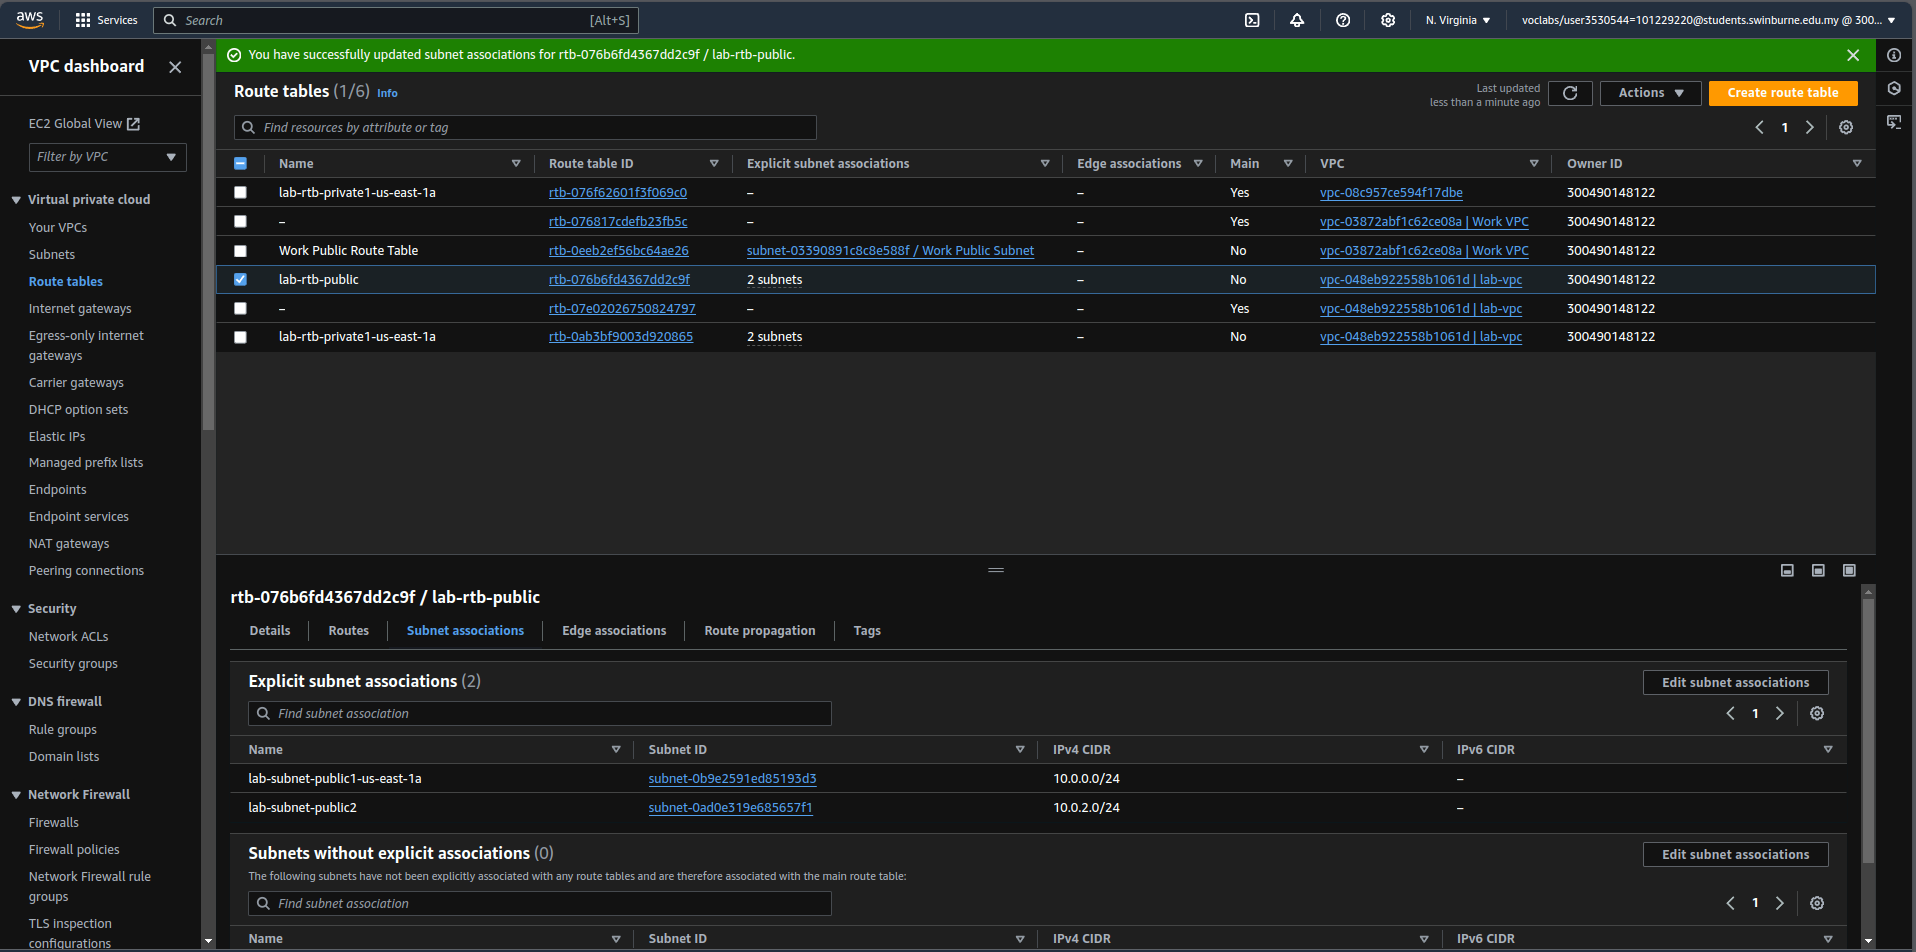
\includegraphics[width=5.8in]{pics/10.png}
    }

\end{enumerate}


\vspace{1cm}

\newpage

\noindent\underline{Task 3: Create a VPC Security Group}

\begin{enumerate}[resume]
    \item Paste screenshot$($s$)$ of the \textbf{Security Groups} screen \\
    \vspace{5mm}

    {\centering
    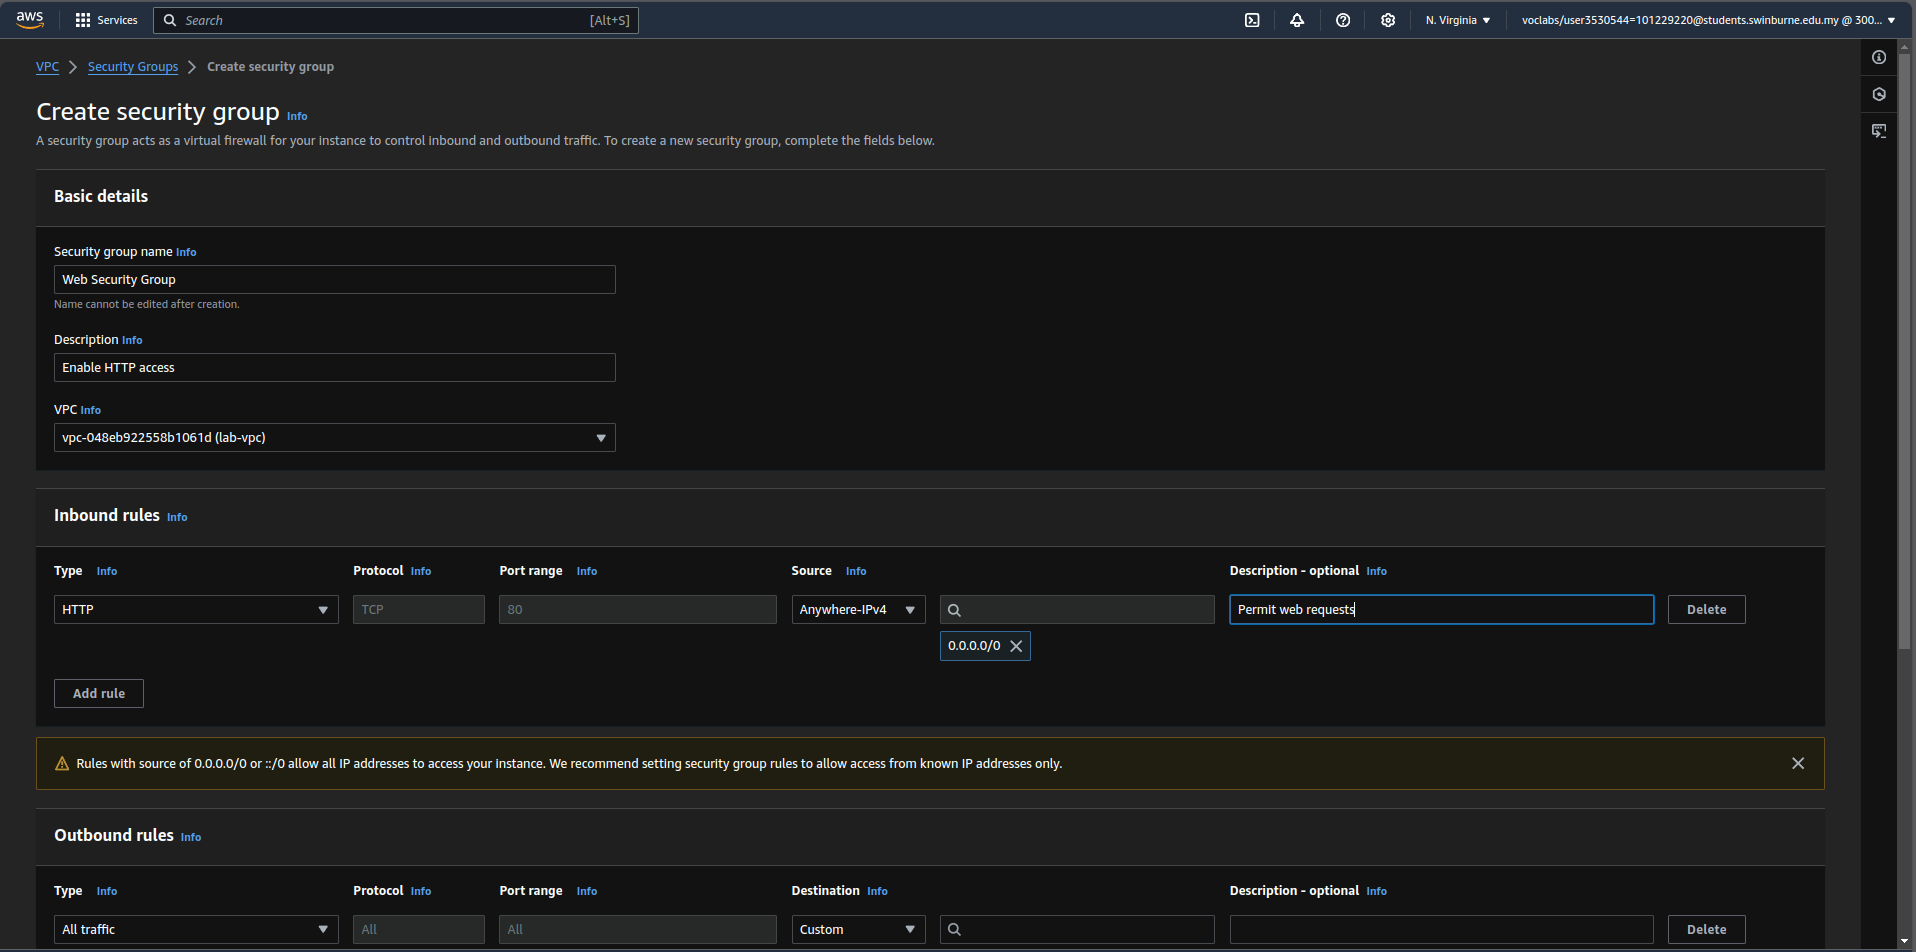
\includegraphics[width=5.8in]{pics/11.png}
    }

    \item Paste screenshot$($s$)$ of the \textbf{Create Security Group} screen (after entering / choosing the \\ appropriate settings) \\
    \vspace{5mm}

    {\centering
    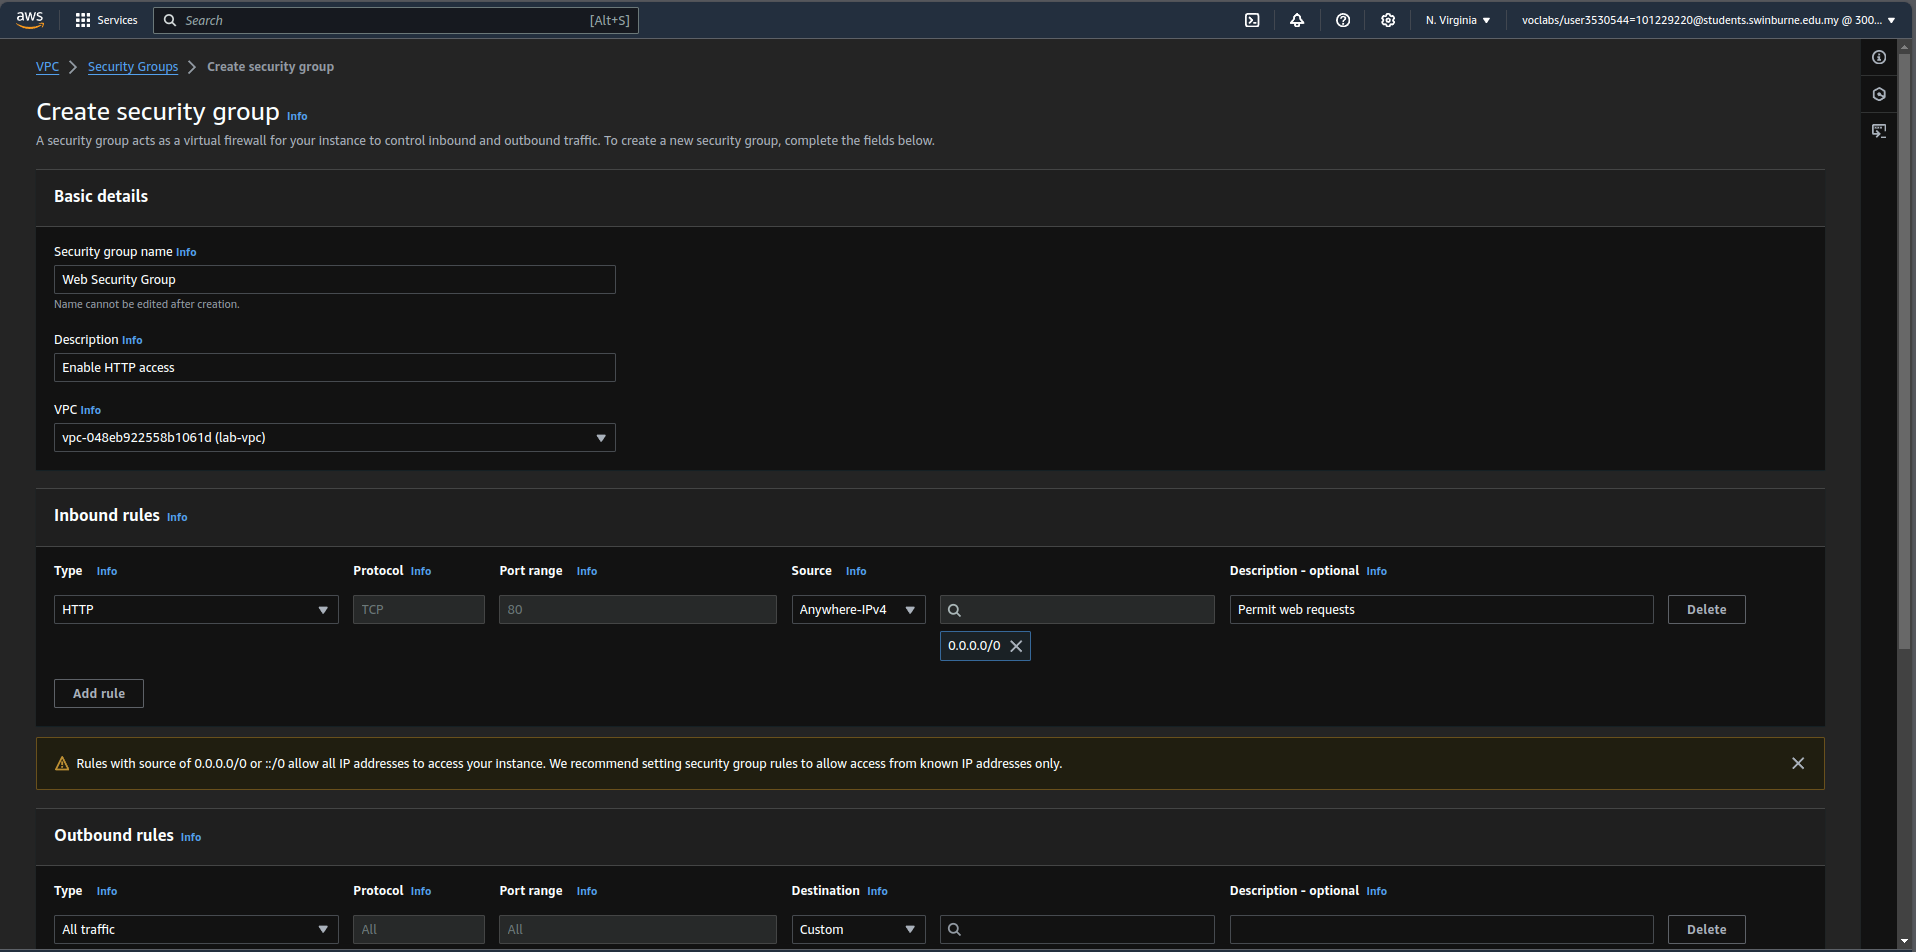
\includegraphics[width=5.8in]{pics/12_a.png}
    }

    {\centering
    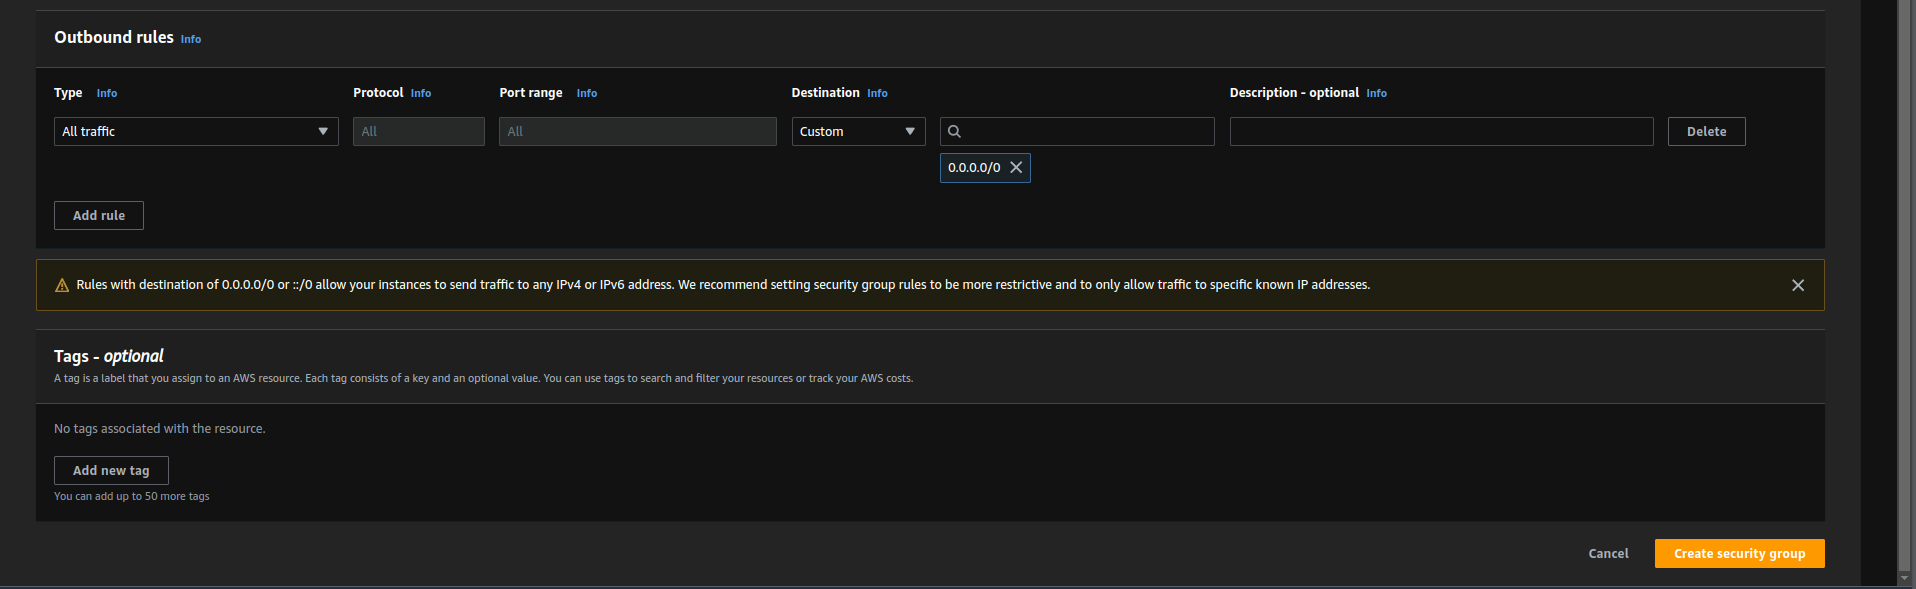
\includegraphics[width=5.8in]{pics/12_b.png}
    }

    
    \item Paste screenshot$($s$)$ of the \textbf{Security Group} screen (showing the inbound rules) \\
    \vspace{1mm}

    {\centering
    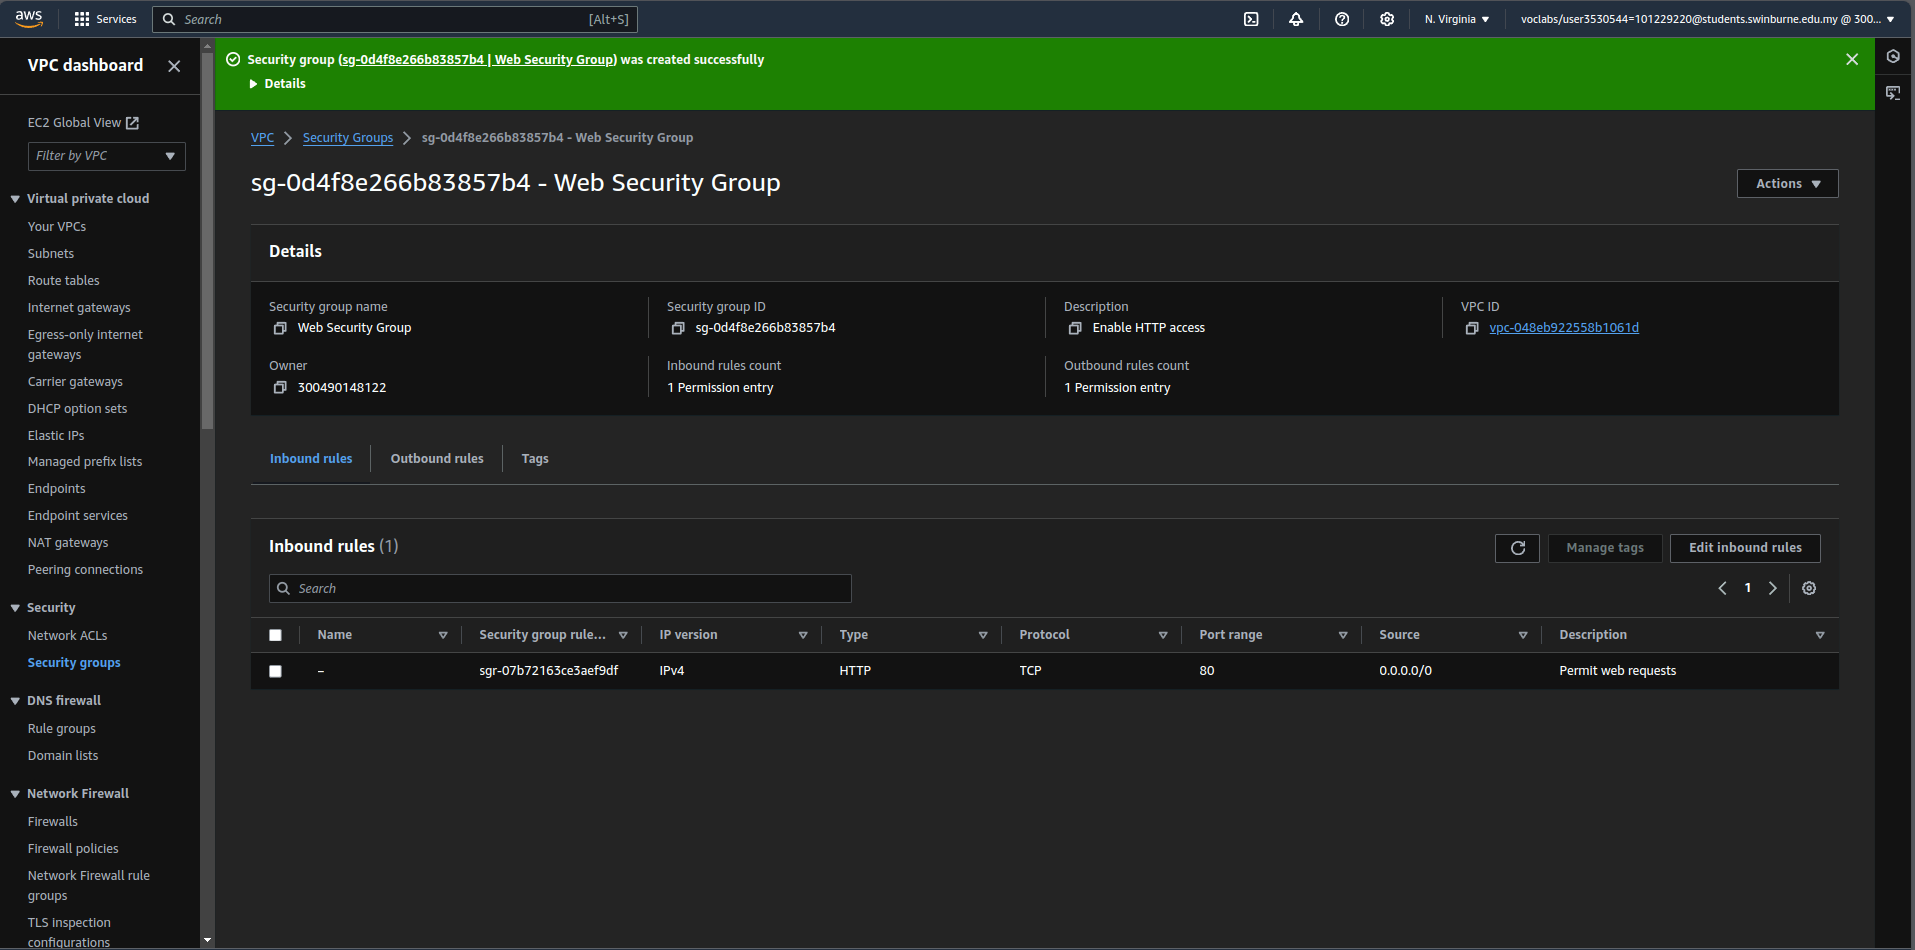
\includegraphics[width=5.8in]{pics/13.png}
    }

\end{enumerate}


\vspace{0.2cm}

\noindent\underline{Task 4: Launch a Web Server Instance}

\begin{enumerate}[resume]
    \item Paste screenshot$($s$)$ of the \textbf{Launch Instance} screen (after entering / choosing the \\ appropriate settings) \\
    \vspace{-0.02mm}

    {\centering
    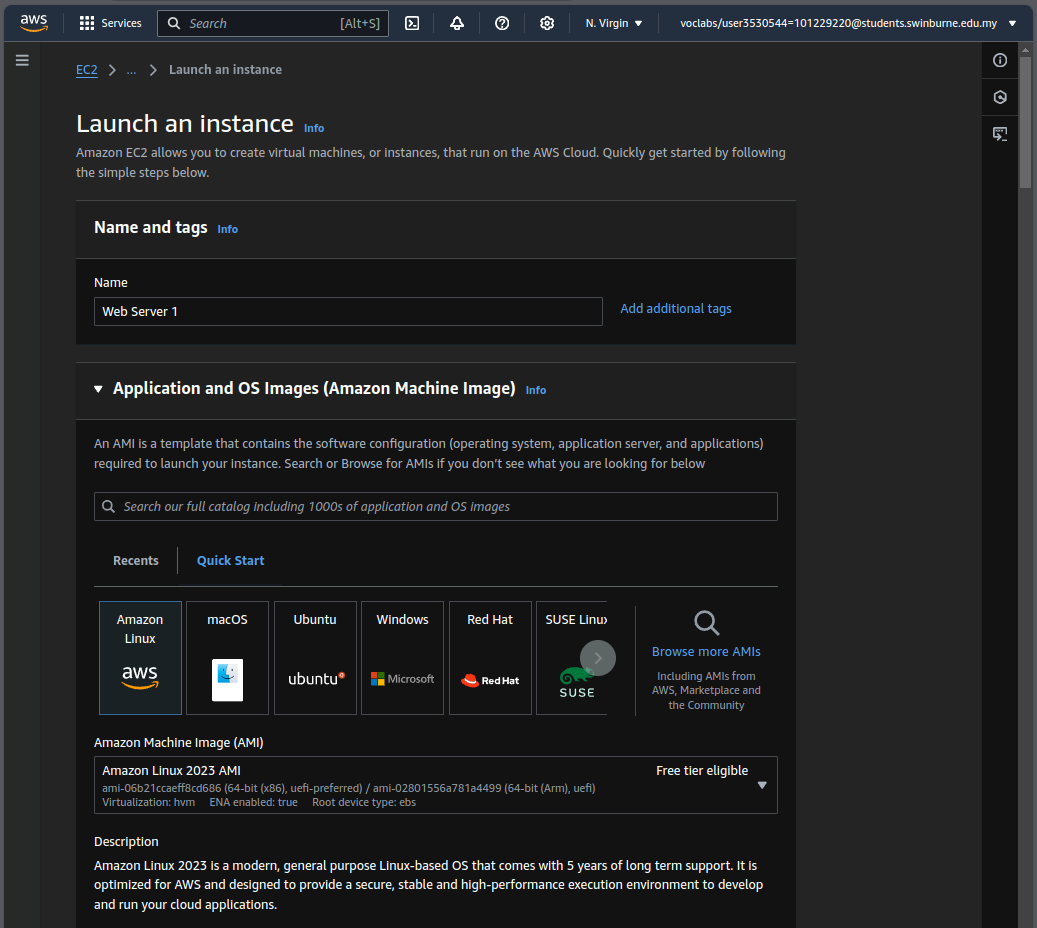
\includegraphics[width=5.8in]{pics/14a.png}
    }

    {\centering
    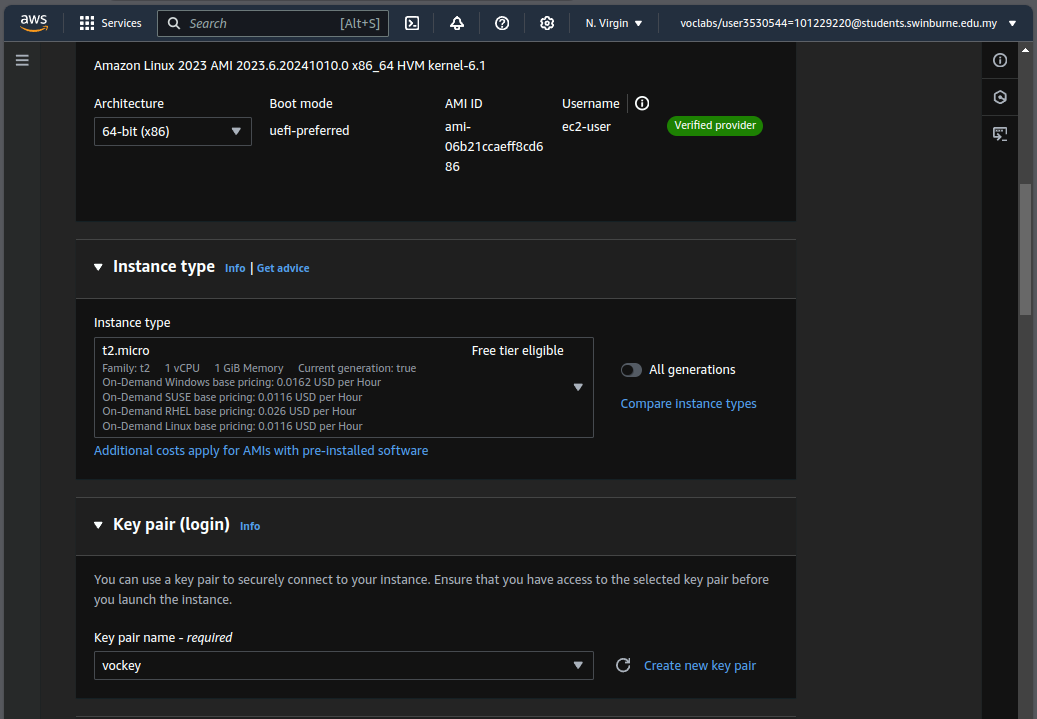
\includegraphics[width=5.8in]{pics/14b.png}
    }


    {\centering
    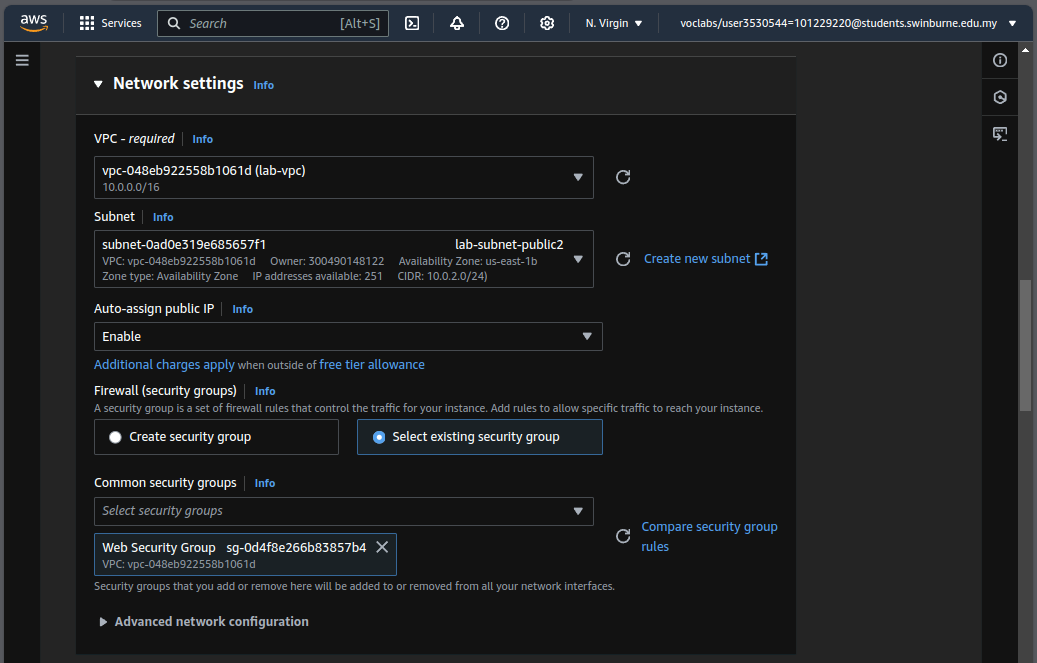
\includegraphics[width=5.8in]{pics/14c.png}
    }


    {\centering
    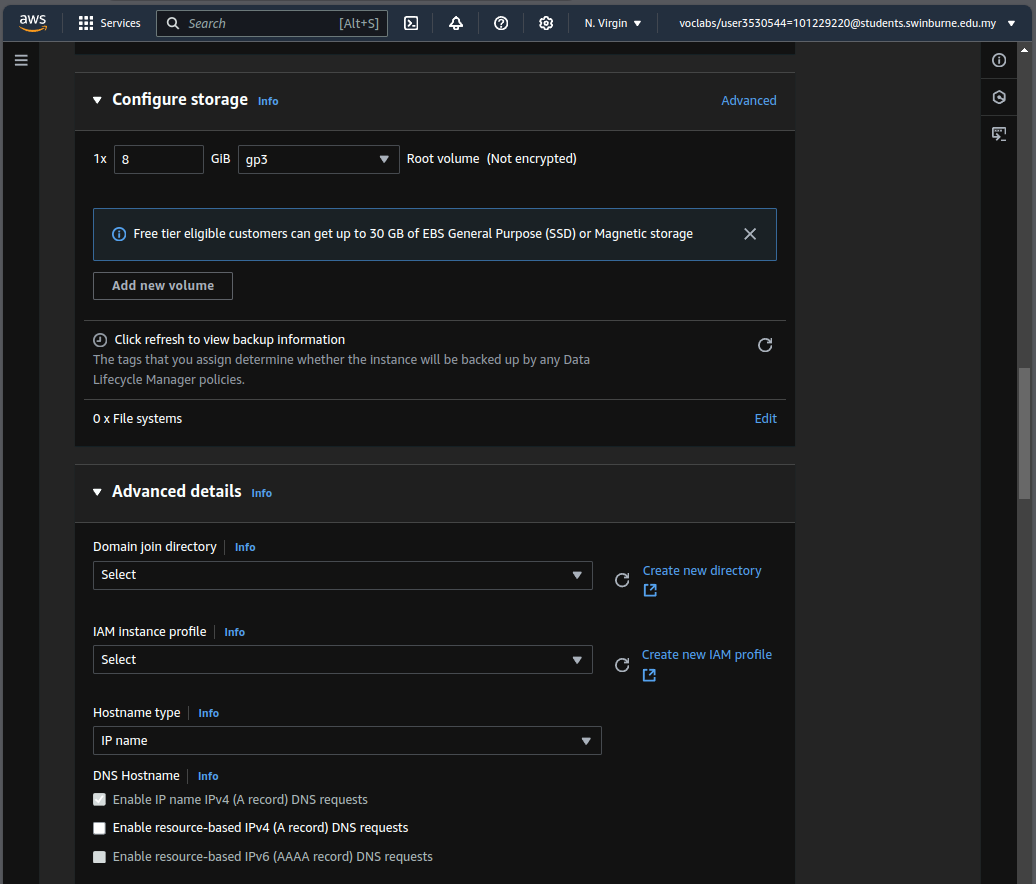
\includegraphics[width=5.8in]{pics/14d.png}
    }


    {\centering
    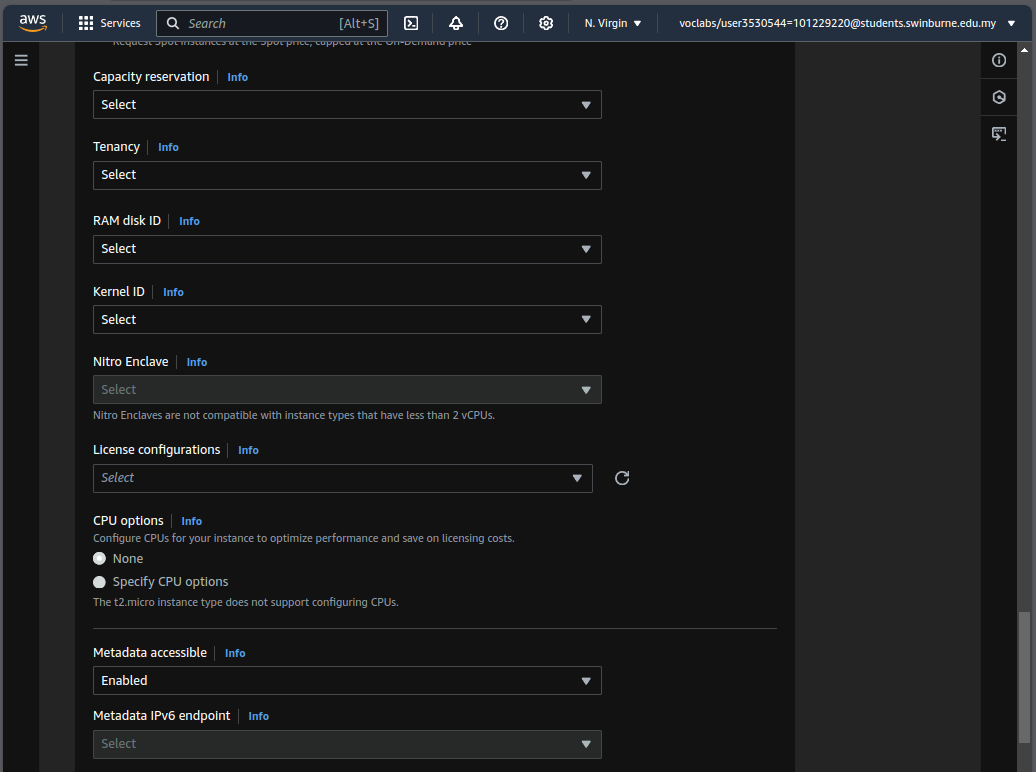
\includegraphics[width=5.8in]{pics/14f.png}
    }


    {\centering
    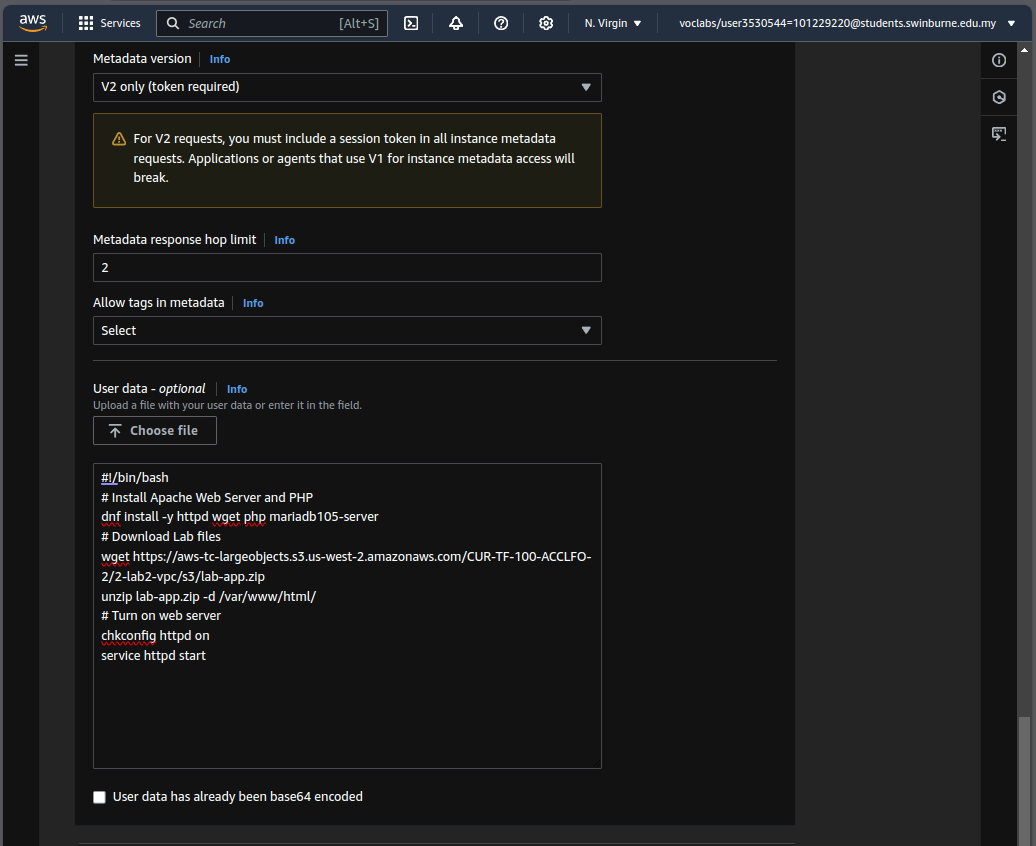
\includegraphics[width=5.8in, height=4.3in]{pics/14g.png}
    }


    {\centering
    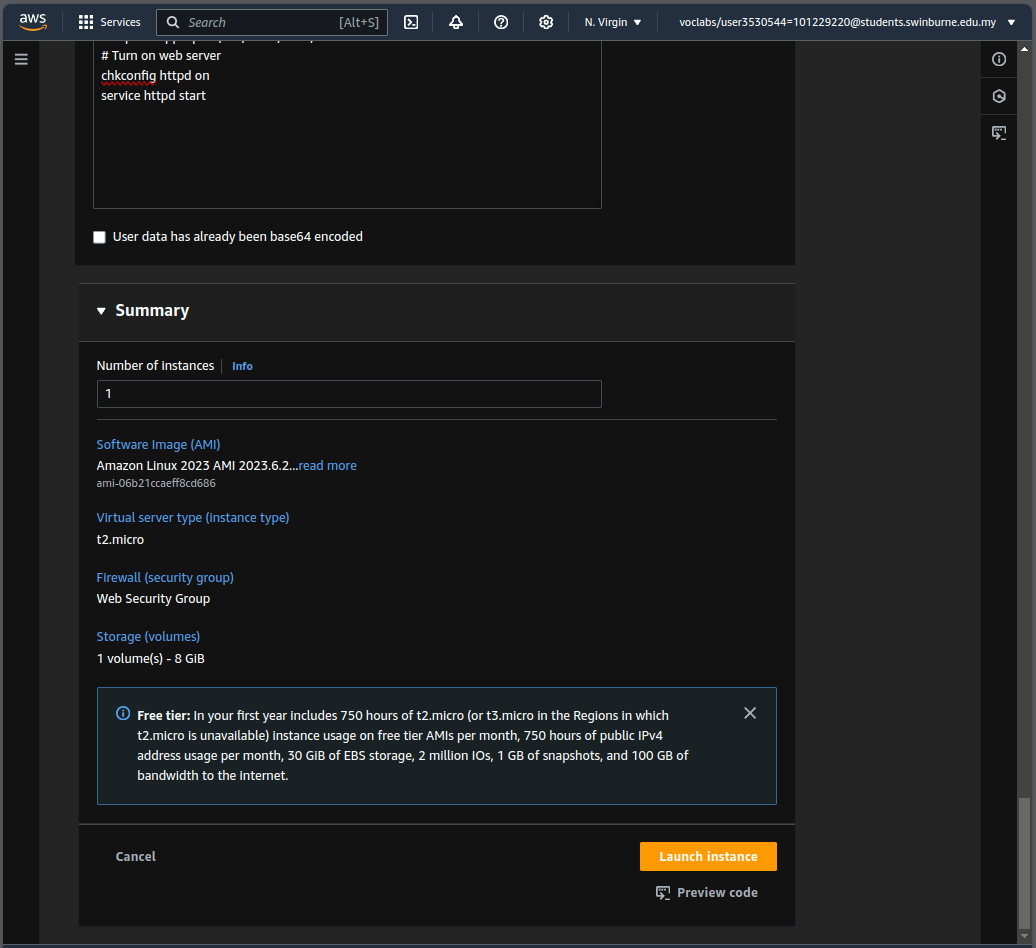
\includegraphics[width=5.8in]{pics/14h.png}
    }
    
    \item Paste screenshot$($s$)$ of the \textbf{Instance Web Page} screen \\
    \vspace{5mm}


    {\centering
    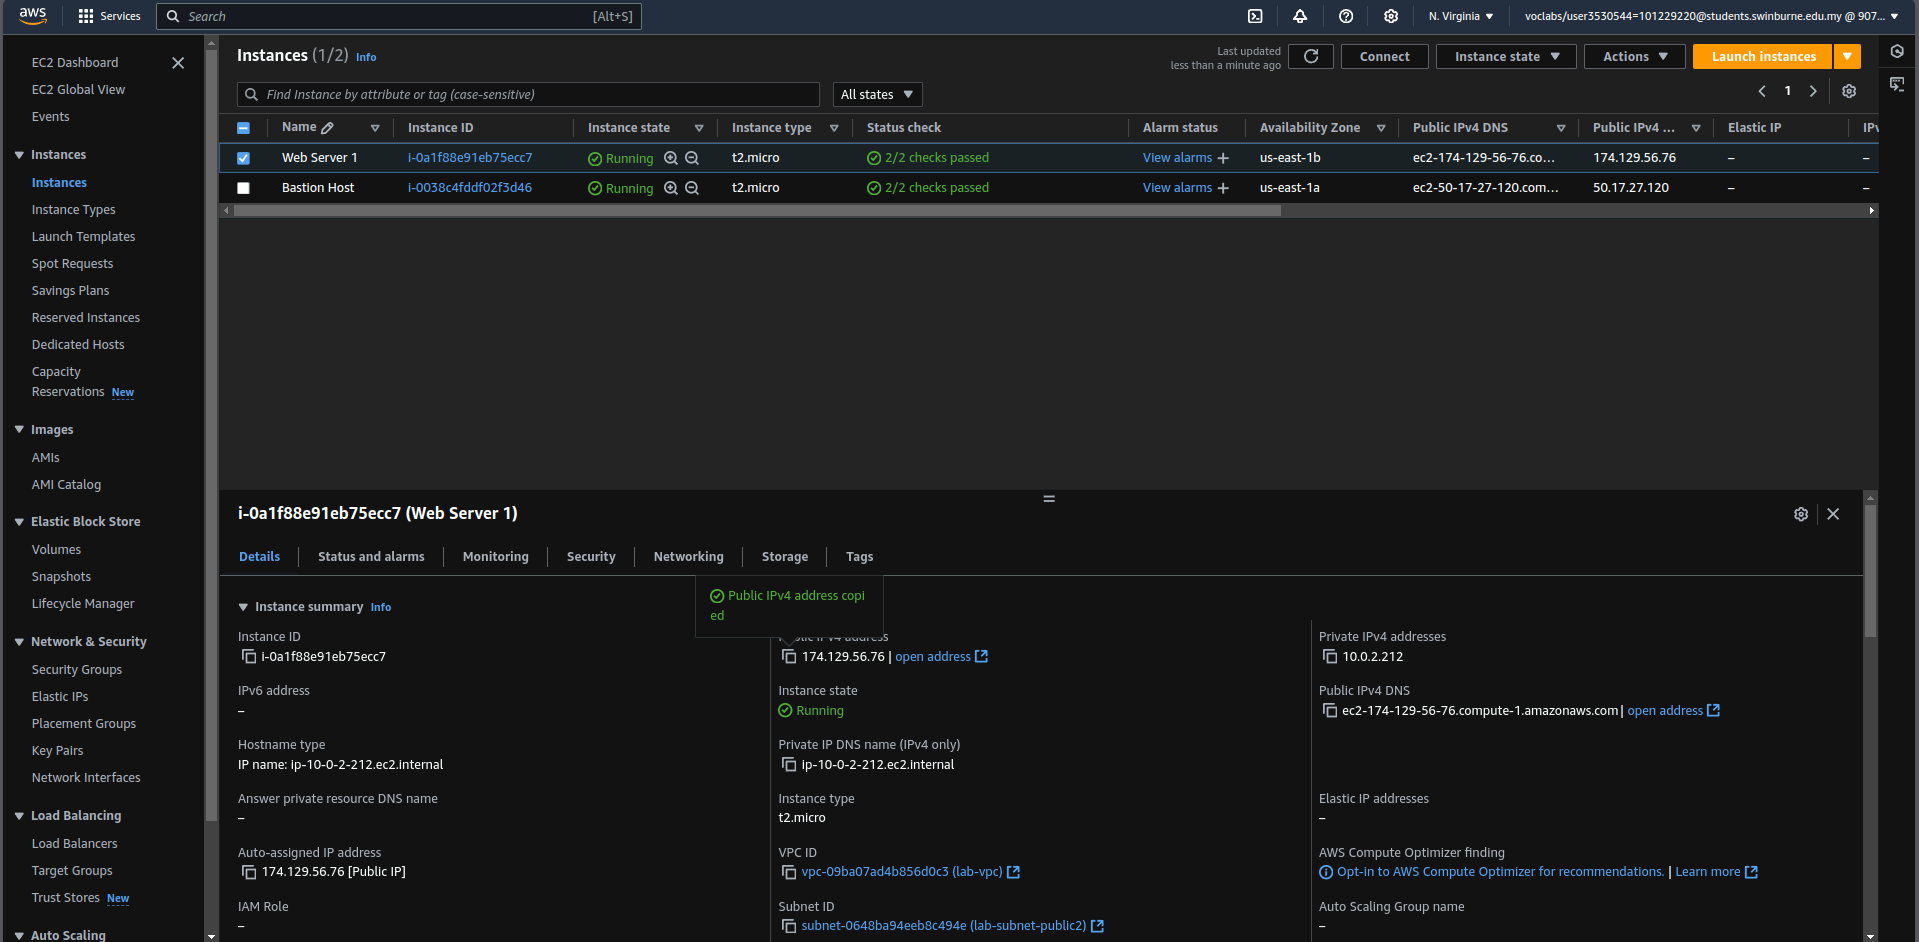
\includegraphics[width=5.8in]{pics/15a.png}
    }
    

    {\centering
    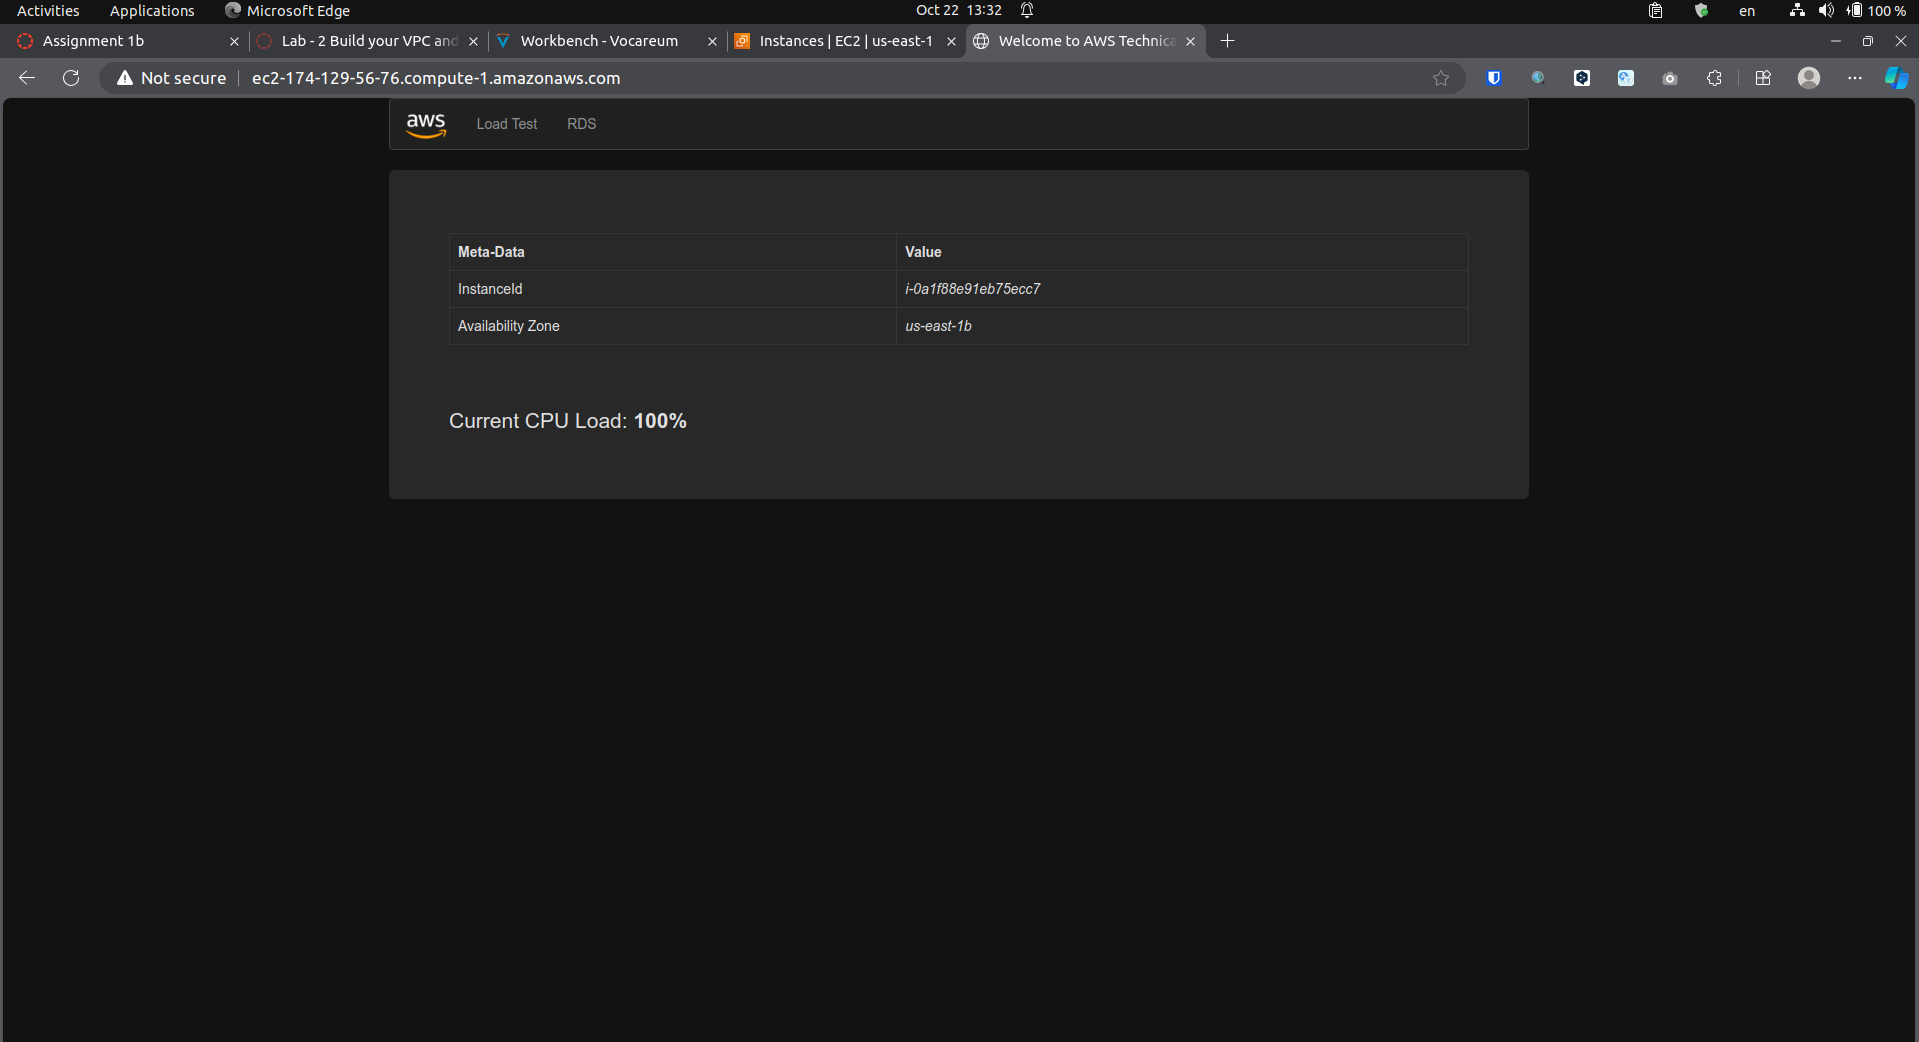
\includegraphics[width=5.8in]{pics/15b.png}
    }
    
        
\end{enumerate}

\newpage

\noindent\underline{Submission Report}

\vspace{0.5cm}

\noindent Paste screenshot (s) of the \textbf{Grades} screen showing your Total score and Tasks \\
\vspace{5mm}


{\centering
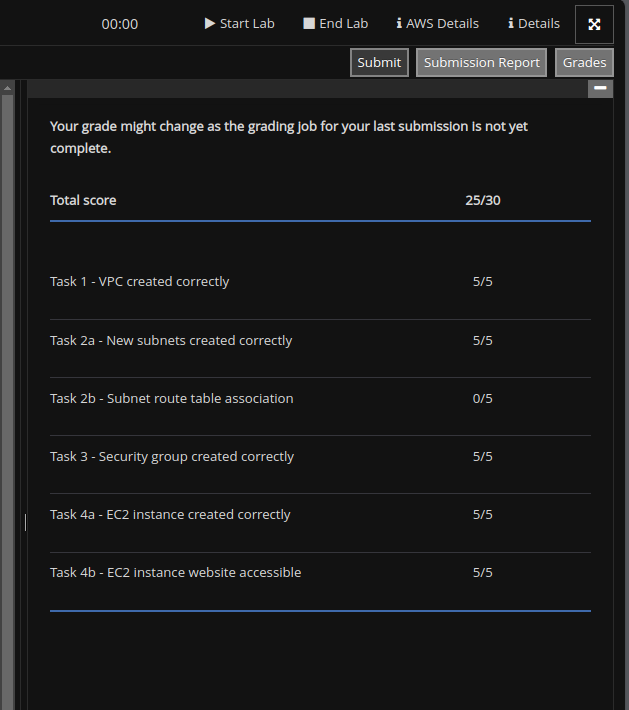
\includegraphics[width=5.8in]{pics/grades.png}
}



\end{document}

